\documentclass[aspectratio=169]{beamer}

\usepackage{amsmath, amssymb, amsxtra, amsthm, amsfonts}
\usetheme{moloch}
\usecolortheme{beaver}
\setbeamertemplate{footline}
{
  \leavevmode%
  \hbox{%
    \begin{beamercolorbox}[wd=.5\paperwidth,ht=2.25ex,dp=1ex,center]{author in head/foot}%
      \usebeamerfont{author in head/foot}\insertsection
    \end{beamercolorbox}%
    \begin{beamercolorbox}[wd=.5\paperwidth,ht=2.25ex,dp=1ex,right]{date in head/foot}%
      \usebeamerfont{date in head/foot}\inserttitle\hspace*{2em}
      \insertframenumber{} / \inserttotalframenumber\hspace*{2ex}
    \end{beamercolorbox}}%
  \vskip0pt%
}
\makeatother

\usepackage[english]{babel}
\usefonttheme{serif}

\usepackage{mathtools}
\usepackage{graphicx}
\usepackage{bm}
\usepackage{color}
\usepackage[dvipsnames,table]{xcolor}
\usepackage{tikz}
\usepackage{stanli}
\usepackage{verbatim}
\usepackage{tikz}
\usetikzlibrary{shapes,calc,through,3d,patterns}
\usetikzlibrary{decorations.pathreplacing}
\usetikzlibrary{arrows.meta,calc,positioning}

\usepackage{pgfplots}
\usepackage{siunitx} % For formatting numbers
\usepackage{hyperref}
\hypersetup{colorlinks=true,linkcolor=darkred}
\usepackage{multicol}
\usepackage[absolute,overlay,]{textpos}
\usepackage{pgfplots}
\pgfplotsset{width=10cm,compat=1.9}
\usepackage{subcaption}
\usepackage{multirow}
\usepackage{bbding}
\usepackage{arydshln}
\usepackage{mathtools}
\usepackage{tcolorbox}
\usepackage{animate}

\textblockorigin{80mm}{45mm}


\newtheorem{thm}{Theorem}
\newtheorem{cor}[thm]{Corollary}
\newtheorem{prop}[thm]{Proposition}
\newtheorem{lem}[thm]{Lemma}
\theoremstyle{remark}
\newtheorem*{rem}{Remark}

%Block def
\definecolor{darkred}{rgb}{0.6,0,0}
\setbeamertemplate{blocks}[rounded][shadow=false]
\setbeamercolor{block title}{bg=darkred!15,fg=black}
\setbeamercolor{block body}{bg=darkred!5,fg=black}

\setbeamercolor{itemize item}{fg=darkred}
\setbeamercolor{itemize subitem}{fg=darkred}
\setbeamercolor{itemize subsubitem}{fg=darkred}
\setbeamercolor{enumerate item}{fg=darkred}
\setbeamercolor{button}{bg=gray!30,fg=darkred}

\setbeamertemplate{itemize item}[square]
\setbeamertemplate{itemize subitem}[circle]
\setbeamertemplate{itemize subsubitem}[triangle]
\setbeamertemplate{enumerate items}[circle]
\setbeamercolor{item projected}{bg=darkred}

\newcommand{\bolddelta}{\boldsymbol\delta}
\newcommand{\boldxi}{\boldsymbol\xi}
\DeclareMathOperator*{\A}{\text{\raisebox{-0.2cm}{\Huge A}}}




\title{Strong and weak forms}
\subtitle{Linear elastodynamics}
\author{ME473 Dynamic finite element analysis of structures}
\institute{Stefano Burzio}
\date{2025}

\begin{document}
\usenavigationsymbolstemplate{}
{\setbeamertemplate{footline}{}

  \frame{\titlepage
    \begin{tikzpicture}[overlay, remember picture]
      \node[anchor=north east, xshift=-.9cm] at (current page.north east) {
\includegraphics[width=2cm]{../images/epfl_logo.png}};
      \node[anchor=south east, xshift=-.87cm, yshift=.05cm] at (current page.south east)  {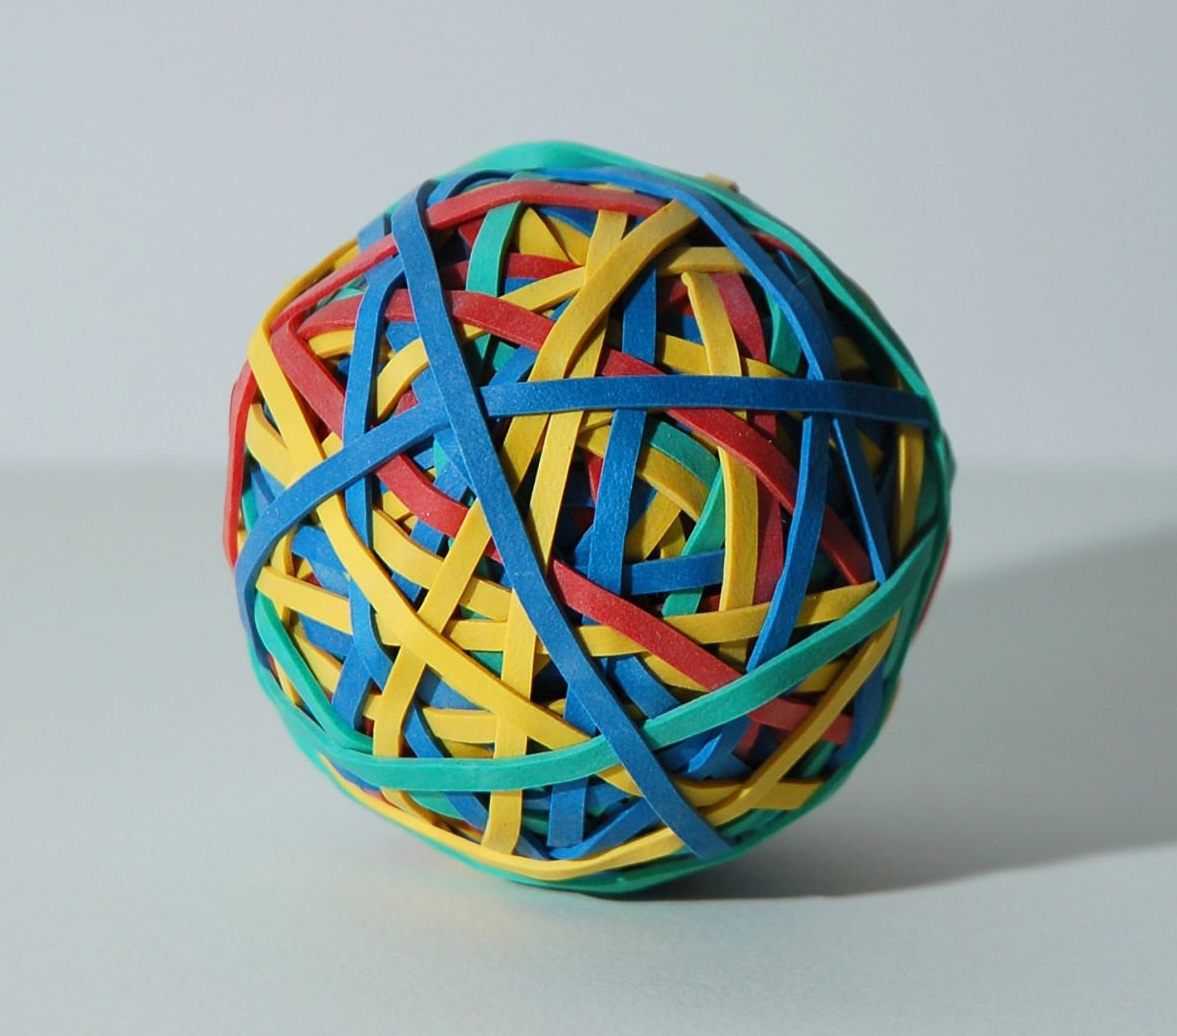
\includegraphics[width=5cm]{../images/rubber_band_ball.jpg}};
    \end{tikzpicture}
  }

  {%background 
    \setbeamertemplate{background canvas}{
\begin{tikzpicture}
        \useasboundingbox (0,0) rectangle (\paperwidth,\paperheight);
        \fill [color=darkred!80] (0.5\paperwidth,0) rectangle (\paperwidth,\paperheight);
      \end{tikzpicture}}



    \begin{frame}
      \begin{columns}
        % Left column with images
        \column{0.55\textwidth}
        \vspace{0.5cm}

        \hspace{0.1cm} 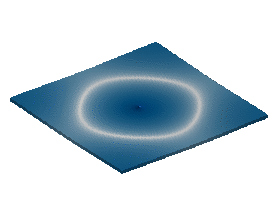
\includegraphics[width=2.5cm]{../images/modePlate1} \hspace{1cm} 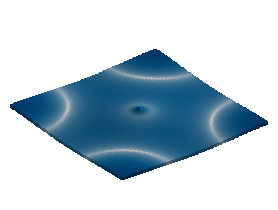
\includegraphics[width=2.5cm]{../images/modePlate2}

        \hspace{0.1cm} 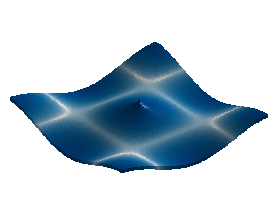
\includegraphics[width=2.5cm]{../images/modePlate3}  \hspace{1cm} 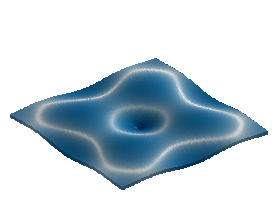
\includegraphics[width=2.5cm]{../images/modePlate4}

        \hspace{0.1cm} 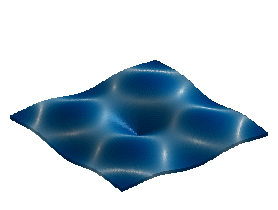
\includegraphics[width=2.5cm]{../images/modePlate5}  \hspace{1cm} 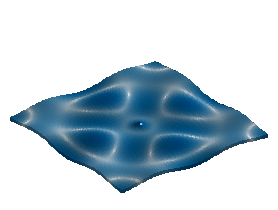
\includegraphics[width=2.5cm]{../images/modePlate6}

        \hspace{0.1cm} 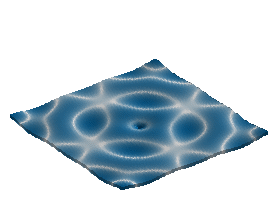
\includegraphics[width=2.5cm]{../images/modePlate7}  \hspace{1cm} 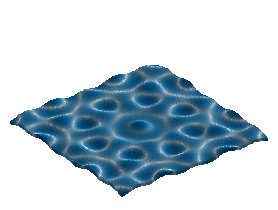
\includegraphics[width=2.5cm]{../images/modePlate8}

        \hspace{0.2cm}\tiny (Credit: \href{https://nojigon.webs.upv.es/simulations_plate.php}{\textcolor{darkred}{Noé Jiménez})}

        % Right column with red background and text
        \column{0.45\textwidth}
        \parbox{\linewidth}{%
          \textbf{\textcolor{white}{\large Linear:}} \textcolor{white}{infinitesimally small deformations relative to the solid's size.} \\[0.9cm]
          \textbf{\textcolor{white}{\large Elasticity:}} \textcolor{white}{deformable material that returns to its original shape and size when the forces causing the deformation are removed.} \\[0.9cm]
          \textbf{\textcolor{white}{\large Dynamics:}} \textcolor{white}{study bodies in motion under the influence of time-dependent loads applied to them.}
        }
      \end{columns}
    \end{frame}
  }

  \begin{frame}
    \textbf{\large Summary}
    \begin{itemize}
      \item Underlying hypothesis and notations
      \item Equilibrium equations
      \item Strong formulation of equilibrium equations
      \item Weak formulation of equilibrium equations
      \item Example 1: longitudinal vibrations of bars
      \item Example 2: transversal vibrations of beams
    \end{itemize}
    \vspace{.5cm}

    \textbf{\large Recommended readings}
    \begin{enumerate}
      \item Gmür, Dynamique des structures (§2.1 and §2.2)
      \item Gmür, Méthode des éléments finis (§5.1 and §5.2)
      \item Neto et al., Engineering Computation of Structures (§1.1, §1.3 and §2.1)
    \end{enumerate}
  \end{frame}
}

\section{Underlying hypothesis and notations}

\begin{frame}{Hypothesis and notations}
  \begin{columns}[T]
    \begin{column}{.69\textwidth}
      \begin{itemize}
        \item Inertial orthonormal reference frame $O(x,y,z)$. \\ Sometimes will use $O(x_{1},x_{2},x_{3})$.
        \item Continuous three-dimensional deformable finite (compact) \textbf{body} with volume $\Omega$ and surface $\Gamma$.
        \item \textbf{Material}: continuous and homogenous.
        \item \textbf{Deformations}: small (proportional to stress).
        \item Continuous and derivable time-dependent (\emph{unknown}) \textbf{displacement field}:
              $$\mathbf u(\mathbf x,t)=\begin{bmatrix}u_1(\mathbf  x,t)\\ u_2(\mathbf  x,t)\\ u_3(\mathbf  x,t) \end{bmatrix}$$
              where $\mathbf  x\in\bar\Omega$ and $t\in[0,T]$.
      \end{itemize}
    \end{column}\hspace{-1.5cm}
    \begin{column}{.4\textwidth}
      \vspace{1cm}
      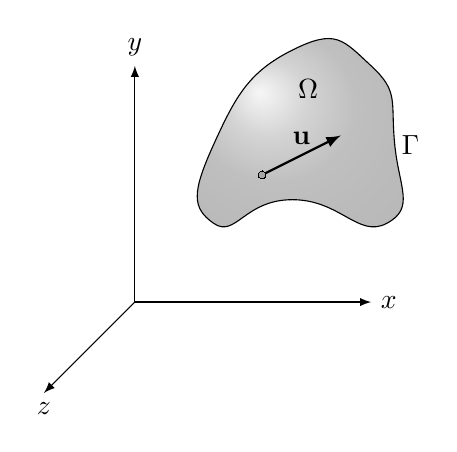
\begin{tikzpicture}
        \draw[-latex] (0,0,0) -- (3,0,0) node[right]{$x$};
        \draw[-latex] (0,0,0) -- (0,3,0) node[above]{$y$};
        \draw[-latex] (0,0,0) -- (0,0,3) node[below]{$z$};
        % Draw the potato-like shape
        \shade [ball color= gray!50!black, opacity=.3] plot [thick,smooth cycle, tension=1] coordinates  {(1,2) (2,3.2) (3,3) (3.3,2) (3.2,1) (2,1.3) (1,1)};
        \draw plot [thick,smooth cycle, tension=1] coordinates {(1,2) (2,3.2) (3,3) (3.3,2) (3.2,1) (2,1.3) (1,1)};
        % Label the region Omega	
        \node at (2.2,2.7) {$\Omega$};
        % Label the boundary Gamma
        \node at (3.5,2) {$\Gamma$};
        \draw[thick,-latex] (2,2,1) to node[midway,above]{$\mathbf u$} (3,2.5,1);
        \node[draw,shape=circle,fill=black!35,minimum size=1mm,line width=0mm,inner sep=0] at (2,2,1) {};
      \end{tikzpicture}
    \end{column}
  \end{columns}
\end{frame}

\begin{frame}{Stress and strain tensors}
  \begin{columns}[T]
    \begin{column}{.33\textwidth}
      \small\centering \textbf{Stress tensor}
      $$\boldsymbol{\sigma}(\mathbf x,t)=\begin{bmatrix}\sigma_{11}(\mathbf x,t)\\ \sigma_{22}(\mathbf x,t)\\ \sigma_{33}(\mathbf x,t)\\ \sigma_{23}(\mathbf x,t)\\ \sigma_{31}(\mathbf x,t)\\ \sigma_{12}(\mathbf x,t)\end{bmatrix}$$
    \end{column}
    \hfill
    \begin{column}{.33\textwidth}\vspace{-0.5cm}
      \begin{center}
        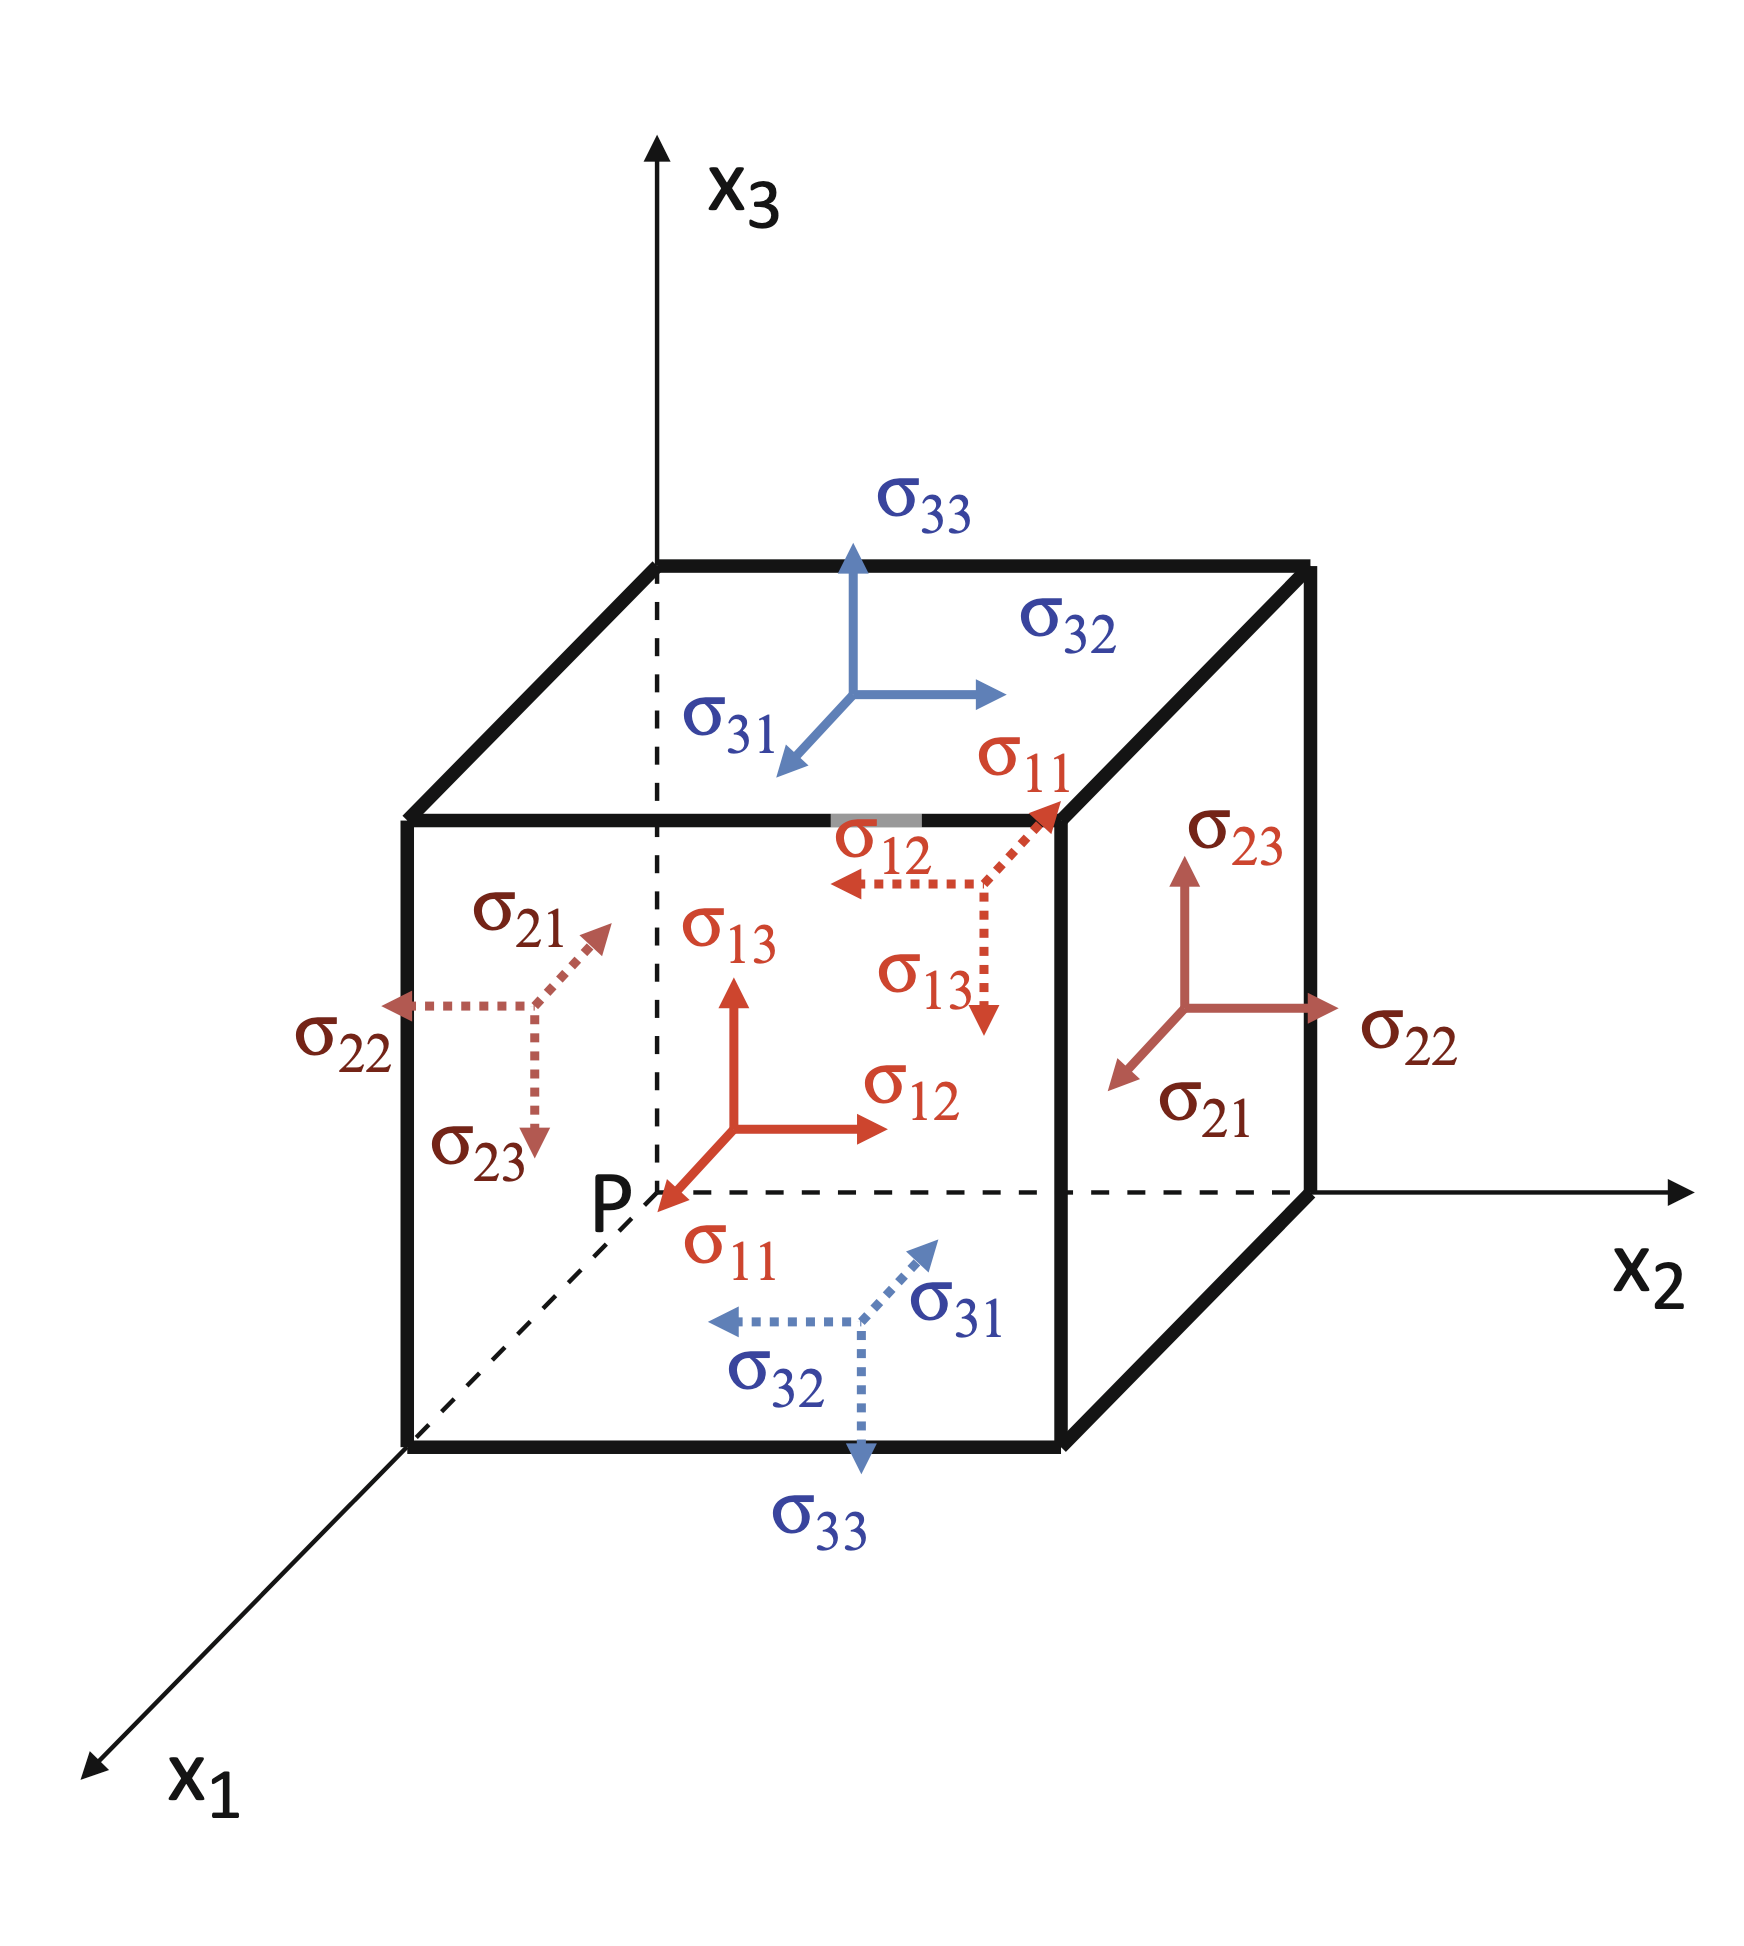
\includegraphics[width=2.5cm]{../images/stressComponents.png}

        \noindent{\tiny\emph{Credit: Neto et al.}}
      \end{center}
    \end{column}
    \hfill
    \begin{column}{.33\textwidth}
      \small\centering \textbf{Strain tensor}
      $$\boldsymbol{\varepsilon}(\mathbf x,t)=\begin{bmatrix}\varepsilon_{11}(\mathbf x,t)\\ \varepsilon_{22}(\mathbf x,t)\\ \varepsilon_{33}(\mathbf x,t)\\ 2\varepsilon_{23}(\mathbf x,t)\\ 2\varepsilon_{31}(\mathbf x,t)\\ 2\varepsilon_{12}(\mathbf x,t)\end{bmatrix}$$
    \end{column}
  \end{columns}
  \vspace{4pt}\noindent\color{darkred}\rule{\linewidth}{0.1mm}\vspace{-12pt}
  {\footnotesize
    \begin{itemize}
      \item \textbf{Stress} expresses the internal forces that neighboring particles of a material exert on each other (SI units of Pascal.)
      \item \textbf{Strain} is defined as relative deformation, compared to a reference position configuration (SI units of meter per meter.)
      \item First index specifies the normal of the surface on which the stress/strain is acting, the second index specifies the direction of the stress/strain.
      \item if $i\neq j$ then $\sigma_{ij}=\tau_{ij}$ (shear stress) and $2\varepsilon_{ij}=\gamma_{ij}$ (engineering shear strain).
      \item Symmetric tensors: $\tau_{ij}=\tau_{ji} $ (Cauchy’s stress theorem) and $\gamma_{ij}=\gamma_{ji}$.
    \end{itemize}
  }
\end{frame}

\begin{frame}{The stress-strain curve}
  \begin{center}
    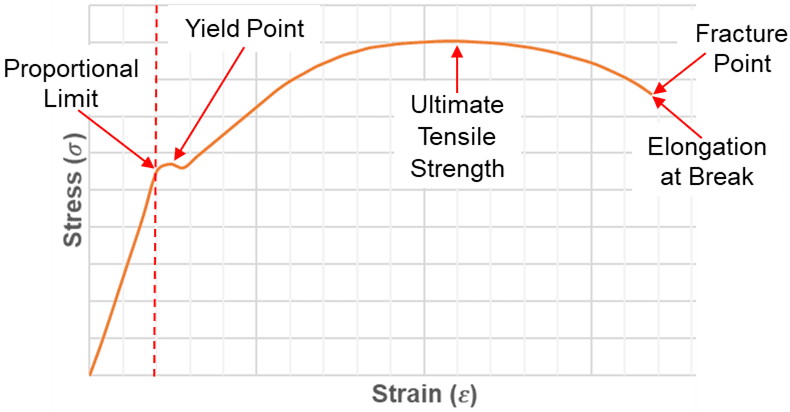
\includegraphics[width=10cm]{../images/strssStrainRelationship.png}
    \newline\noindent{\tiny\emph{Credit: \href{https://www.fidelisfea.com/post/stress-and-strain-what-are-they-and-what-is-their-relationship}{\textcolor{darkred}{Fidelis}}}}
  \end{center}
\end{frame}

\begin{frame}{Generalised Hooke’s law}
  \begin{block}{}
    The constitutive stress-strain relationship of linear elasticity is given by the Hooke’s law:
    $$\boldsymbol\sigma(\mathbf x,t)       = \mathbf C\,\boldsymbol\varepsilon(\mathbf x,t)$$
    or equivalently
    $$\boldsymbol\varepsilon(\mathbf x,t)  = \mathbf S\, \boldsymbol\sigma(\mathbf x,t)$$
    where $\mathbf C$ is called the \emph{stiffness (constitutive) material matrix} and $\mathbf S=\mathbf C^{-1}$ the \emph{compliance matrix}.
  \end{block}
  \footnotesize
  \begin{table}[htbp]
    \centering
    \renewcommand{\arraystretch}{1.5}
    \begin{tabular}{lcc}
        \hline
        & \textbf{Stiffness $C$} & \textbf{Compliance $S$} \\
        \hline        
        \textbf{Measures}
        & Resistance to deformation
        & Deformability \\
        
        \textbf{Units}
        & $\mathrm{Pa}$
        & $\mathrm{Pa}^{-1}$ \\
        
        \textbf{Large value means}
        & Stiff
        & Compliant       \\  
        \hline
    \end{tabular}
\end{table}
\end{frame}

\begin{frame}{1 - Anisotropic materials}
  \textbf{No symmetry}: these materials have properties that vary with direction and do not have symmetry. Their stiffness differ depending on the axis of measurement.
  \vspace{0.2cm}
  {\small $$\mathbf S=\begin{bmatrix} s_{11} & s_{12} & s_{13} & s_{14} & s_{15} & s_{16} \\ s_{21} & s_{22} & s_{23} & s_{24} & s_{25} & s_{26} \\ s_{31} & s_{32} & s_{33} & s_{34} & s_{35} & s_{36} \\ s_{41} & s_{42} & s_{43} & s_{44} & s_{45} & s_{46}\\ s_{51} & s_{52} & s_{53} & s_{54} & s_{55} & s_{56}\\ s_{61} & s_{62} & s_{63} & s_{64} & s_{65} & s_{66} \end{bmatrix}$$}
  \begin{itemize}
    \item Most of the elements are non-zero, the matrix $\mathbf S$ is considered dense.
    \item 21 independent constants (symmetry).
  \end{itemize}
\end{frame}

\begin{frame}{2 - Orthotropic materials}
  \textbf{Three planes of symmetry}: a special case of anisotropic materials where properties vary along three mutually perpendicular directions. These materials have three different principal material properties along three axes.
  \vspace{0.2cm}
  {\small $$\mathbf S=\begin{bmatrix} 1/E_1 & -\nu_{21}/E_2 & -\nu_{31}/E_3 & 0 & 0 & 0 \\  -\nu_{12}/E_1 & 1/E_2  & -\nu_{32}/E_3  & 0 & 0 & 0 \\ -\nu_{13}/E_1 & -\nu_{23}/E_2 & 1/E_3 & 0 & 0 & 0 \\ 0 & 0 & 0 & 1/G_{23} & 0 & 0 \\ 0 & 0 & 0 & 0 & 1/G_{31} & 0 \\ 0 & 0 & 0 & 0 & 0 & 1/G_{12} \end{bmatrix}$$}
  \begin{itemize}
    \item $E_{i}$ is the Young's modulus along axis $Ox_{i}$.
    \item $G_{ij}$ is the shear modulus in direction $Ox_{i}$ on the plane whose normal is $Ox_{j}$.
    \item $\nu_{ij}$ is the Poisson's ratio that corresponds to a contraction in direction $Ox_{j}$ when an extension is applied in direction $Ox_{i}$.
    \item 9 independent constants.
  \end{itemize}
\end{frame}

\begin{frame}{3 - Isotropic materials}
  \textbf{Infinite planes of symmetry}: these materials have identical properties in all directions. Their mechanical and physical properties do not change regardless of the direction in which they are measured.
  \vspace{0.2cm}
  {\small $$\mathbf S=\begin{bmatrix} 1/E & -\nu/E & -\nu/E & 0 & 0 & 0 \\  -\nu/E & 1/E  & -\nu/E  & 0 & 0 & 0 \\ -\nu/E & -\nu/E & 1/E & 0 & 0 & 0 \\ 0 & 0 & 0 & 1/G & 0 & 0 \\ 0 & 0 & 0 & 0 & 1/G & 0 \\ 0 & 0 & 0 & 0 & 0 & 1/G \end{bmatrix}$$}
  \begin{itemize}
    \item $E$ is the Young's modulus, $G$ is the shear modulus, and $\nu$ is the Poisson's ratio.
    \item Only two independent constants since $E=2G(1+\nu)$.
  \end{itemize}
\end{frame}

\begin{frame}
  \frametitle{Strain-displacement relationship}
  \vspace{-.4cm}{\footnotesize\begin{itemize}
      \item Both normal strain and shear strain can be interpreted as measures of displacement change per unit length.
      \item Strain is obtained by derivatives of displacements for small deformations.
      \item The strain-displacement relation can be written in the three equivalent forms as follows:
    \end{itemize}}
  \vspace{-.4cm}
  \begin{columns}[T]
    \hspace{1.5cm}\begin{column}{.5\textwidth}
      \begin{block}{Kinematics}
        \begin{enumerate}
          \item[a)] $\boldsymbol\varepsilon(\mathbf x,t) =\boldsymbol\nabla\mathbf u(\mathbf x,t)$
                \vspace{0.2cm}
          \item[b)] $\begin{bmatrix}\varepsilon_{11}\\ \varepsilon_{22}\\ \varepsilon_{33}\\ 2\varepsilon_{23}\\ 2\varepsilon_{31}\\ 2\varepsilon_{12}\end{bmatrix}=\begin{bmatrix} \partial_x & 0 & 0 \\ 0 & \partial_y & 0 \\ 0 & 0 & \partial_z \\ 0 & \partial_z & \partial_y \\ \partial_z & 0 & \partial_x  \\ \partial_y & \partial_x & 0 \end{bmatrix}\begin{bmatrix}u_{1}\\ u_{2}\\ u_{3}\end{bmatrix}$
                \vspace{0.2cm}
          \item[c)] $\varepsilon_{ii}=\partial_{x_{i}}u_i$ and $2\varepsilon_{ij}=\partial_{x_{i}}u_j+\partial_{x_{j}}u_i$
        \end{enumerate}
      \end{block}
    \end{column}
    \begin{column}{.5\textwidth}
      \begin{center}
        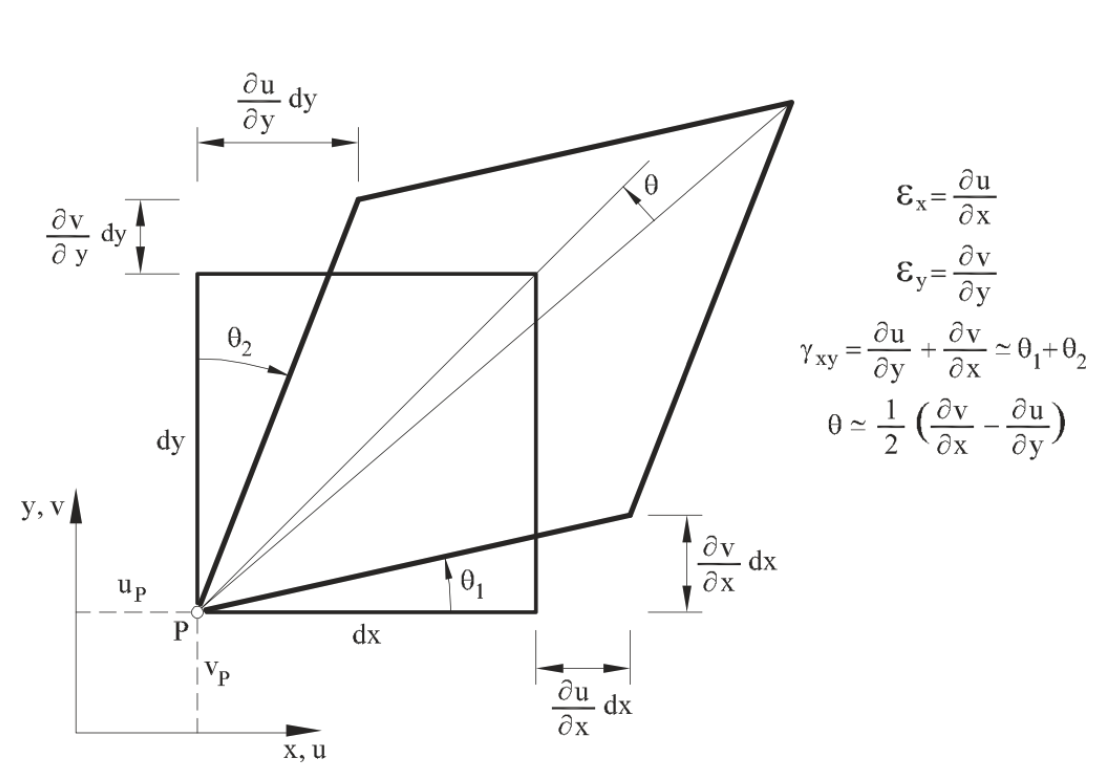
\includegraphics[width=6cm]{../images/strainDisplacementRelationship.png}
        \newline\noindent{\tiny\emph{Credit: Neto et al.}}
      \end{center}
    \end{column}
  \end{columns}
\end{frame}

\section{Equilibrium equations}

\begin{frame}
  \frametitle{Differential equations of motion}
  \begin{columns}[T]
    \begin{column}{.8\textwidth}
      \small
      \begin{itemize}
        \item Consider an infinitely small cube subjected to a force represented by the vector:
              $$\mathbf f(\mathbf x,t)=\begin{bmatrix}f_1(\mathbf x,t)\\ f_2(\mathbf x,t)\\ f_3(\mathbf x,t) \end{bmatrix}.$$
        \item Stress is not uniform. The variation of the stress between two opposite sides is linear and
              $$d\sigma_{ij}=\partial_{x_{k}}\sigma_{ij}\, dx_k$$
              \vspace{-.5cm}
        \item Newton 2nd law of motion taking into account internal forces $\mathbf f^{int}$ is
              $$\mathbf f^{int}(\mathbf x,t)+\mathbf f(\mathbf x,t)=\rho\, \mathbf{\ddot{u}}(\mathbf x,t)\, dx_1dx_2dx_3$$
      \end{itemize}

    \end{column}
    \hfill
    \begin{column}{.28\textwidth}
      \begin{center}
        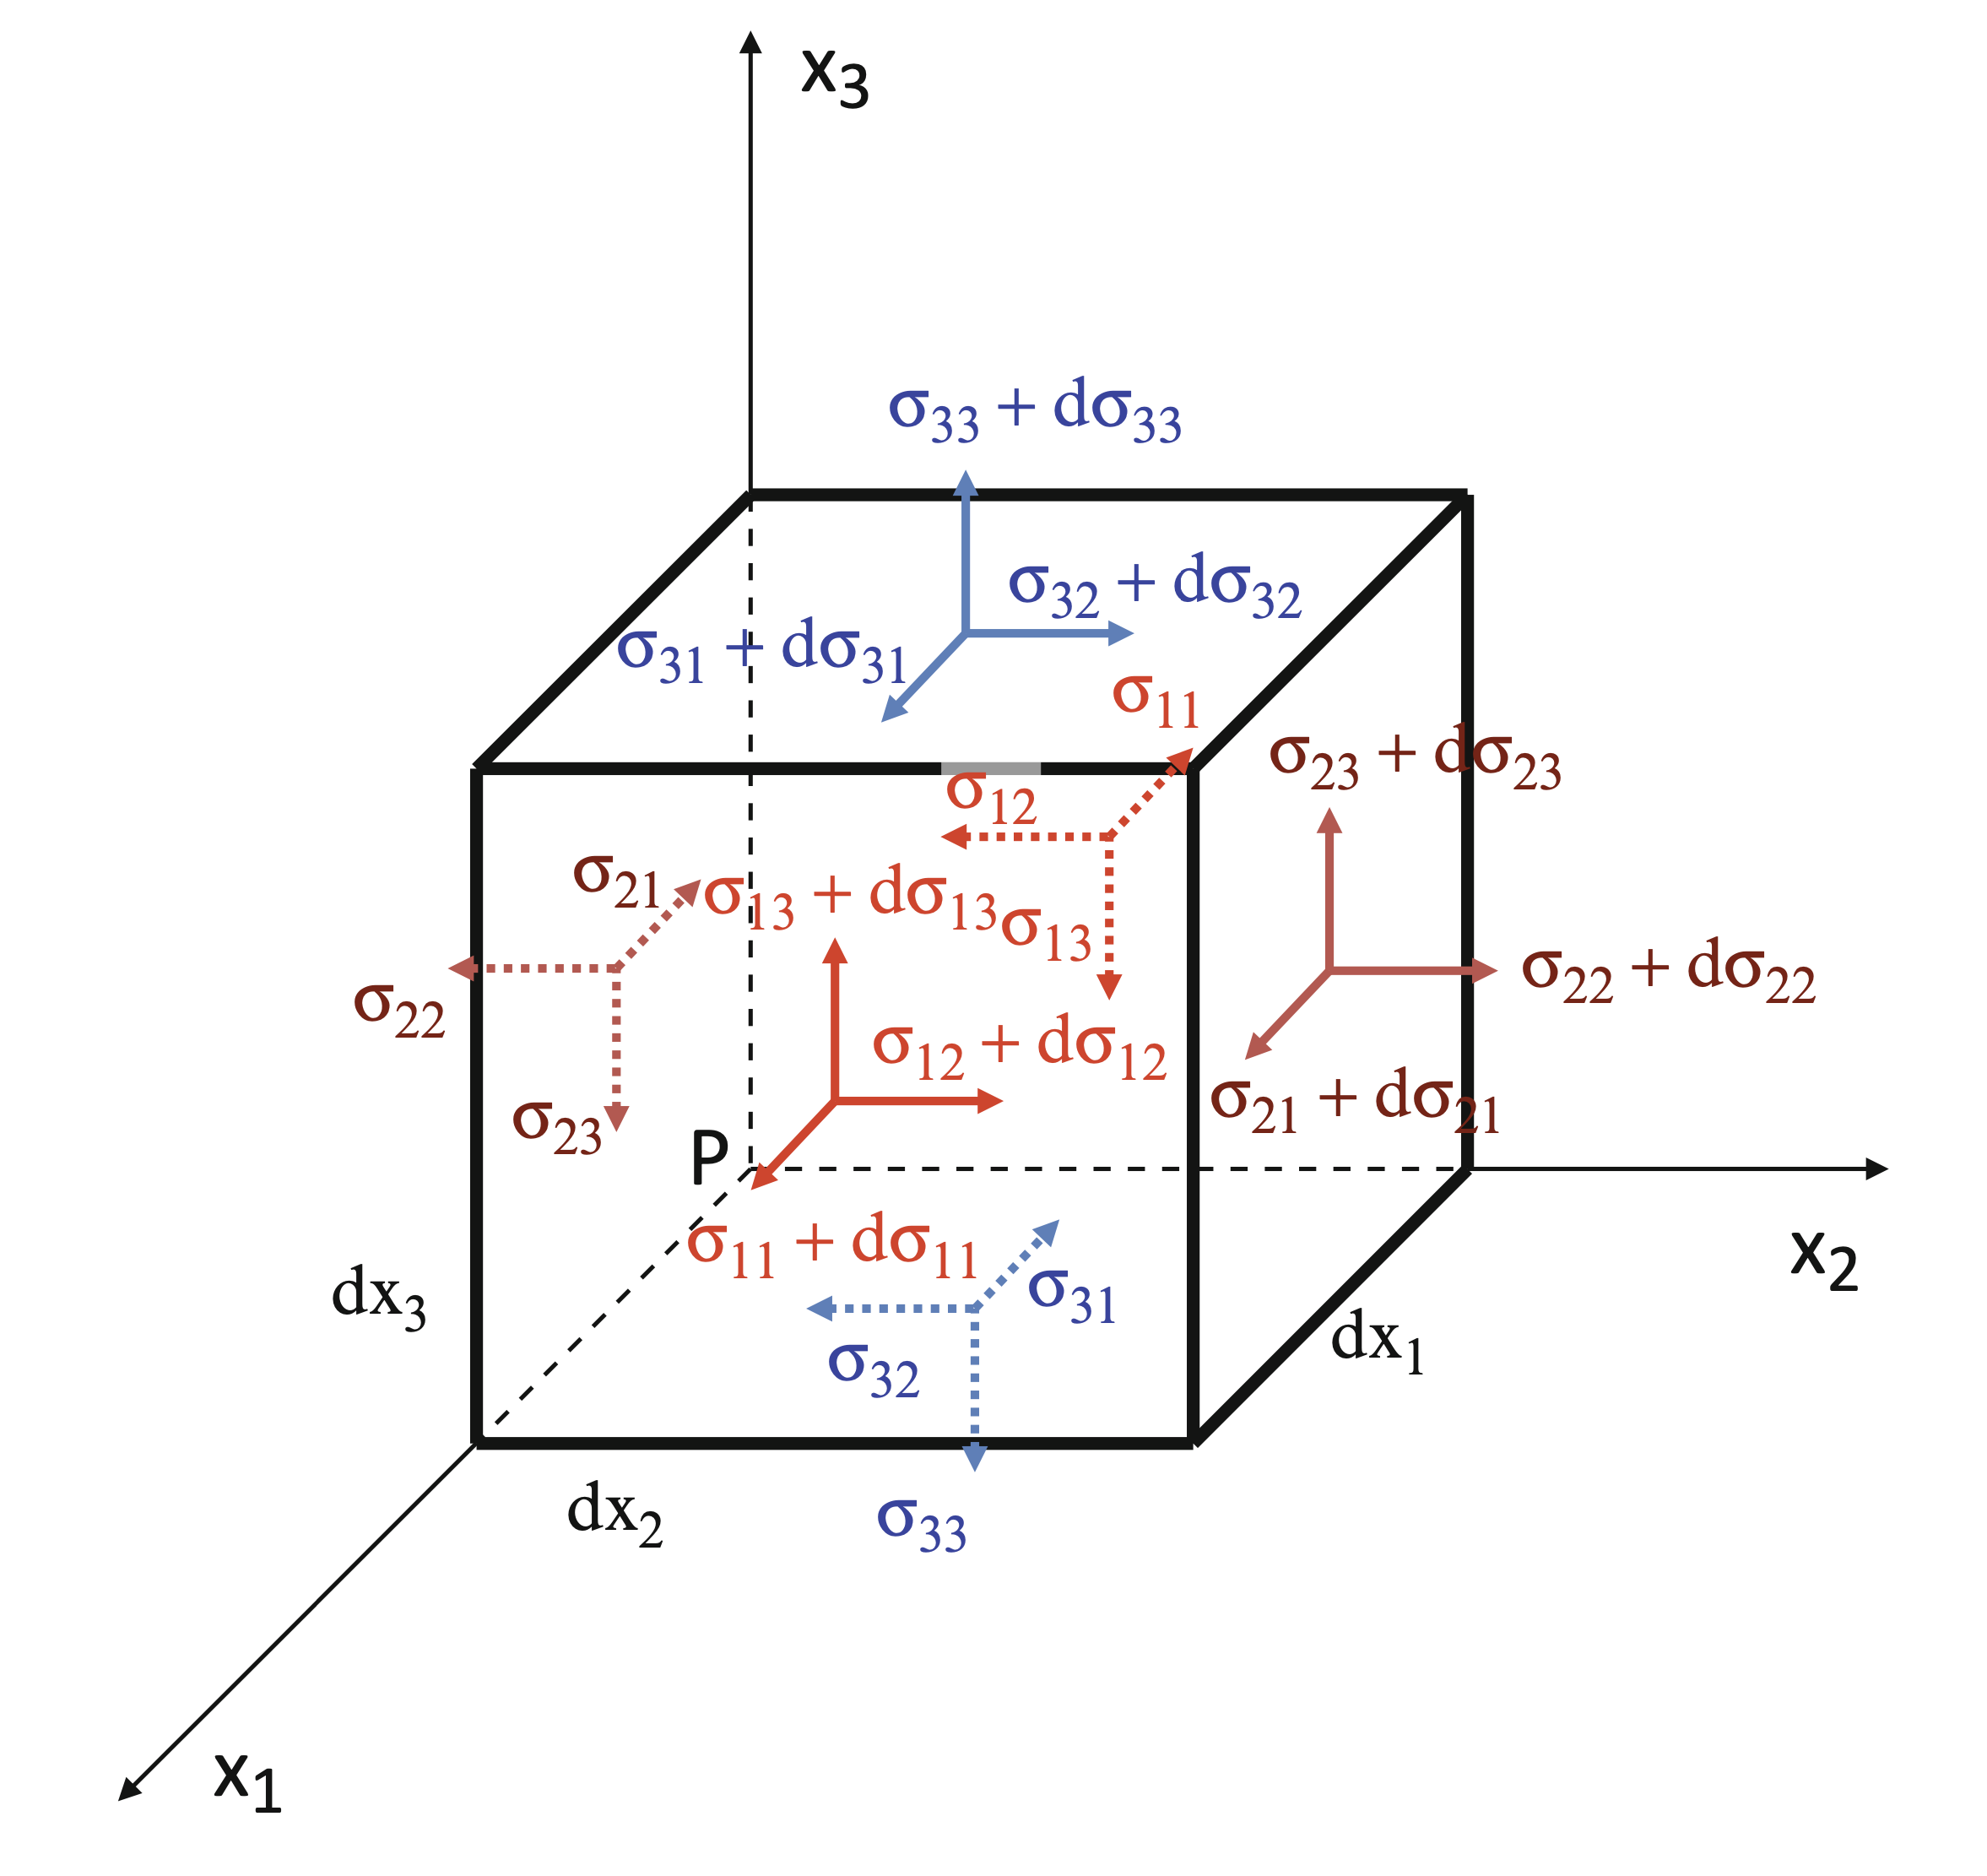
\includegraphics[width=4cm]{../images/diffEqOfMovement}
        \newline\noindent{\tiny\emph{Credit: Neto et al. }}
      \end{center}
    \end{column}
  \end{columns}
  \vspace{.3cm}
  \small $\rho$ is the material density, $\mathbf{\ddot{u}}=\partial_{tt}\mathbf u$ is the acceleration, $dx_1dx_2dx_3$ is the cube's volume.
\end{frame}


{\setbeamercolor{background canvas}{bg=darkred}
\setbeamercolor{block body}{bg=darkred,fg=white}
\setbeamercolor{itemize item}{fg=white}
\begin{frame}{Differential equations of motion}
  \begin{block}{}
    \begin{itemize}
      \item The equilibrium equation of elastodynamics in matrix form is:
            $$\boldsymbol\nabla^T\boldsymbol\sigma(\mathbf x,t)+\mathbf f(\mathbf x,t)=\rho\, \mathbf{\ddot{u}}(\mathbf x,t)$$
      \item Using the strain-displacement relation we can write it in terms of the displacement filed:
            $$\boldsymbol\nabla^T\mathbf C\boldsymbol\nabla\mathbf u(\mathbf x,t)+\mathbf f(\mathbf x,t)=\rho\, \mathbf{\ddot{u}}(\mathbf x,t)$$
    \end{itemize}
  \end{block}
\end{frame}
}

\begin{frame}
  \frametitle{Boundary conditions}
  \small Boundary conditions are appointed for each point on the solid surface $\Gamma=\Gamma_u\cup\Gamma_\sigma$.
  \vspace{-.2cm}
  \begin{columns}[T]
    \begin{column}{.8\textwidth}
      \small
      \begin{itemize}
        \item \textbf{Prescribed displacement:}
              $$\mathbf u=\mathbf{\hat u}\qquad \mbox{on}\  \Gamma_u\times]0,T[$$
              where $\mathbf{\hat u}=[\hat u_1, \hat u_2,\hat u_3]^T$ is the given displacement prescribed on $\Gamma_u$.
        \item \textbf{Prescribed surface force:}
              $$\mathbf N^T\boldsymbol\sigma= \mathbf{\hat f}\qquad \mbox{on}\  \Gamma_\sigma\times]0,T[$$
              $\mathbf{\hat f}=[\hat f_1,\hat f_2,\hat f_3]^T$ is the given surface load prescribed on $\Gamma_\sigma$ and
              $$\mathbf N^T=\begin{bmatrix}n_1 & 0 & 0 & 0 & n_3 & n_2\\ 0 & n_2 & 0 & n_3 & 0 & n_1\\  0 & 0 & n_3 & n_2 & n_1 & 0\\  \end{bmatrix}$$
      \end{itemize}

    \end{column}
    \hfill
    \begin{column}{.28\textwidth}
      \begin{center}
        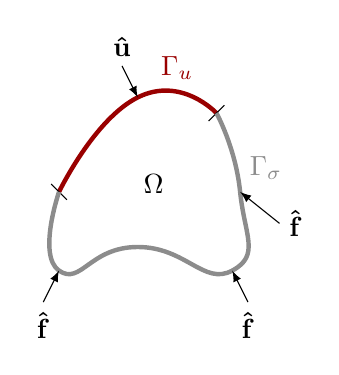
\begin{tikzpicture}
          % Label the region Omega	
          \node at (2.2,2.1) {$\Omega$};
          % Label the boundary Gamma
          \draw[ultra thick, darkred] plot [smooth, tension=1] coordinates {(1,2) (2,3.2) (3,3)};
          \node[darkred, above] at (2.5,3.3) {$\Gamma_u$};
          \draw[thin] (3+0.1,3+0.1) --(3-0.1,3-0.1);
          \draw[thin] (1+0.1,2-0.1) --(1-0.1,2+0.1);
          \draw[latex-]  (2,3.2) --  (2-0.2,3.2+0.4) node[above] {$\mathbf{\hat u}$};
          % Draw part of the boundary Gamma_sigma
          \draw[ultra thick, gray!90] plot [smooth, tension=1] coordinates {(3,3) (3.3,2) (3.2,1) (2,1.3) (1,1) (1,2)};
          \node[gray!90, right] at (3.3,2.3) {$\Gamma_\sigma$};
          \draw[latex-]  (1,1) --  (1-0.2,1-0.4) node[below] {$\mathbf{\hat f}$};;
          \draw[latex-]  (3.2,1) --  (3.2+0.2,1-0.4) node[below] {$\mathbf{\hat f}$};
          \draw[latex-]  (3.3,2) --  (3.3+0.5,2-0.4) node[right] {$\mathbf{\hat f}$};
        \end{tikzpicture}
      \end{center}
    \end{column}
  \end{columns}
  \vspace{.2cm}
  \small $n_{i}$ being the \emph{direction cosines} for the outward-pointing normal $\mathbf n=[n_{1},\, n_{2},\, n_{3}]^T$ to the boundary $\Gamma_{\sigma}$.
\end{frame}

\begin{frame}
  \frametitle{Initial conditions}
  \vspace{-0.3cm}
  The initial conditions are set at $t=0$:
  \vspace{0.3cm}
  \begin{itemize}
    \item \textbf{Imposed initial displacement field:}
          $$\mathbf u(\mathbf x,0)=\mathbf{u_0}(\mathbf x)\qquad \forall \mathbf x\in\Omega$$
    \item \textbf{Imposed initial velocity field:}
          $$\mathbf{\dot u}(\mathbf x,0)=\mathbf{v_0}(\mathbf x)\qquad \forall \mathbf x\in\Omega$$
  \end{itemize}
\end{frame}

\begin{frame}
  \frametitle{Continuum mechanical modelling}
  \begin{center}
    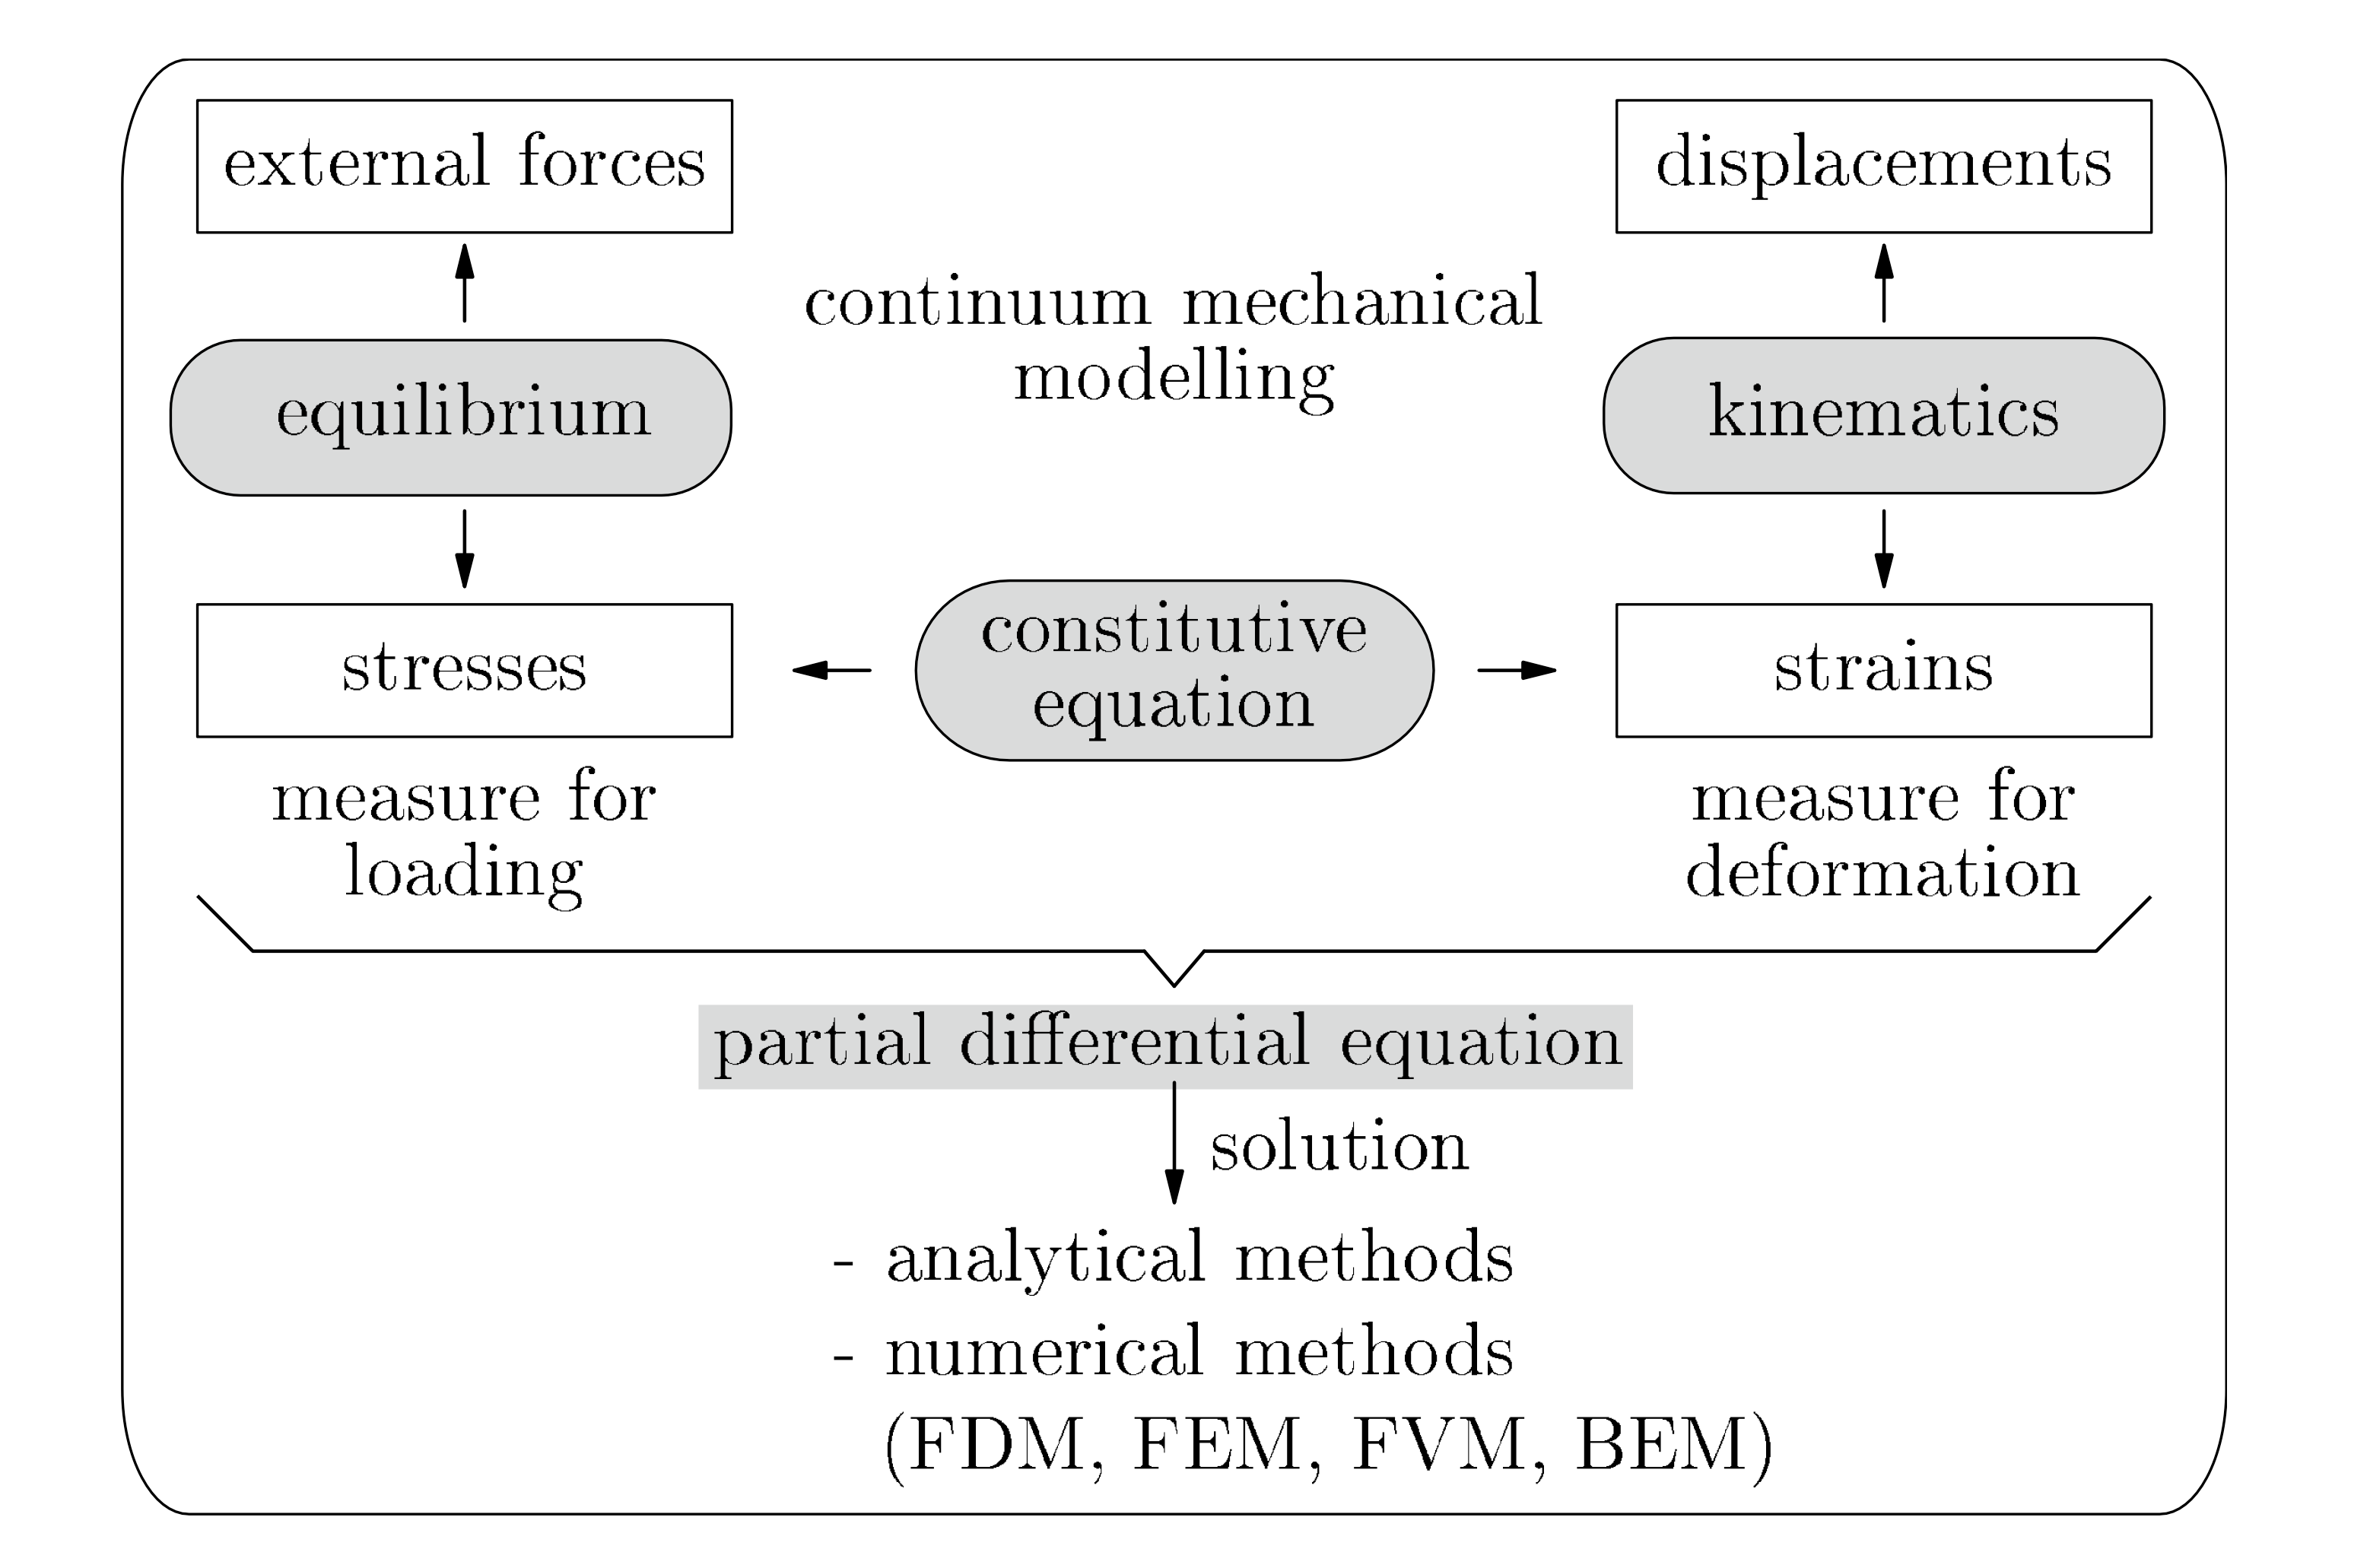
\includegraphics[width=10cm]{../images/contMecaModelling}
  \end{center}
  \noindent{\tiny\emph{Credit: A. Öchsner - PDE for classical structural members}}
\end{frame}

\section{Strong formulation of equilibrium equations}

 {\setbeamercolor{background canvas}{bg=darkred}
  \setbeamercolor{block body}{bg=darkred,fg=white}
  \setbeamercolor{itemize item}{fg=white}
  \begin{frame}{Strong form of elastodynamics}
    \begin{block}{}
      Given a deformable solid $\Omega$ with boundary $\Gamma$, and
      \begin{itemize}
        \item stiffness material matrix $\mathbf C$ and material density $\rho$,
        \item vector of body load $\mathbf f$ applied on $\Omega$,
        \item prescribed boundary displacement $\mathbf{\hat u}$ on $\Gamma_{u}$ and surface load $\mathbf{\hat f}$ on $\Gamma_{\sigma}$,
        \item prescribed initial (at $t=0$) displacement $\mathbf u_{0}$ and initial velocity $\mathbf v_{0}$.
      \end{itemize}
      find the displacement $\mathbf u\in C^{2}(\bar\Omega\times[0,T],\mathbb R^{3})$ such that
      $$\begin{cases}
          \boldsymbol\nabla^T\mathbf C\boldsymbol\nabla \mathbf u+\mathbf f=\rho\, \mathbf{\ddot{u}} & \text{on }\Omega\times]0,T[         \\
          \mathbf u=\mathbf{\hat u}                                                                  & \text{on } \Gamma_u\times]0,T[      \\
          \mathbf N^T\mathbf  C\boldsymbol\nabla\mathbf  u=\mathbf{\hat f}                           & \text{on } \Gamma_\sigma\times]0,T[ \\
          \mathbf u=\mathbf u_0                                                                      & \text{for } t=0                     \\
          \mathbf{\dot u} =\mathbf v_0                                                               & \text{for } t=0                     \\
        \end{cases}$$
    \end{block}
  \end{frame}
 }

\section{Example 1: longitudinal vibrations of bars}

\begin{frame}{Strong form for longitudinal vibrations of bars}
  \vspace{-0.2cm}
  \footnotesize\textbf{Kinematic assumptions:}
  \begin{itemize}
    \item The bar cross-section is infinitely rigid in its own plane, remaining plane after deformation.
    \item Loads, which are uniform in every cross-section, can only be applied axially.
    \item The influence on the axial movement of the bar of lateral displacements due to the Poisson effect is negligible ($\sigma_{22}=\sigma_{33}=0$). Thus the bar can undergo only axial stress $\sigma_{11}$, which is uniform in every cross-section.
  \end{itemize}
  \vspace{-.3cm}
  \begin{columns}
    \column{0.55\textwidth}
    \begin{center}
      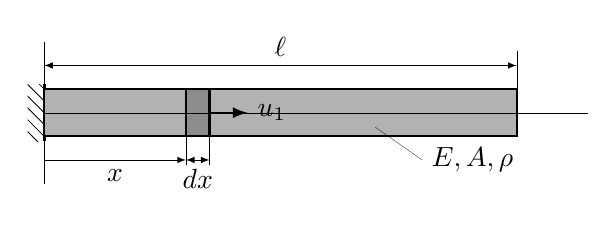
\begin{tikzpicture}[scale=0.6]
        \point{a}{0}{0};
        \support {3}{a}[270];
        % Draw the rectangle
        \filldraw[fill=gray!60, draw=black,thick] (0,-0.5) rectangle (10,0.5);
        \filldraw[fill=gray!90, draw=black,thick] (3,-0.5) rectangle (3.5,0.5);
        \draw[ultra thin] (3,-.5) -- (3,-1.1);
        \draw[ultra thin] (3.5,-.5) -- (3.5,-1.1);
        \draw[latex-latex,ultra thin] (3,-1) to node[midway,below] {$dx$} (3.5,-1);
        \draw[-latex,ultra thin] (0,-1) to node[midway,below] {$x$} (3,-1);
        %axis
        \draw[ultra thin] (0,0) -- (11.5,0);
        \draw[ultra thin] (0,-1.5) -- (0,1.5);
        % length
        \draw[ultra thin] (10,0) -- (10, 1.3) ;
        \draw[latex-latex, ultra thin]  (0,1)  to node[midway,above] {$\ell$}(10,1) ;
        \draw[ultra thin]  (7,-0.3) -- (8,-1) node[right]{$E,A,\rho$};
        \draw[-latex,thick] (3.5,0) to  (4.3,0) node[right]{$u_{1}$};
      \end{tikzpicture}
    \end{center}

    \column{0.25\textwidth}
    {\tiny \begin{itemize}\setlength\itemsep{0.05em}
        \item $A$ cross-sectional area
        \item $E$ Young's modulus
        \item $\rho$ material density
        \item $\ell$ length
      \end{itemize}}
    \column{0.3\textwidth}
    {\tiny \begin{itemize}\setlength\itemsep{0.05em}
        \item $x$ axial coordinate
        \item $u_1(x,t)$ axial displacement
        \item $N_1(x,t)$ normal internal force
        \item $\sigma_{11}(x,t)$ normal stress
        \item $\varepsilon_{11}(x,t)$ normal strain
      \end{itemize}}
  \end{columns}\vspace{-.3cm}
  \begin{columns}
    \column{0.22\textwidth}
    \begin{block}{}
      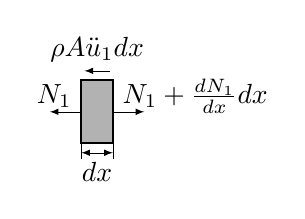
\begin{tikzpicture}[scale=0.4]
        % Draw the rectangle
        \filldraw[fill=gray!60, draw=black,thick] (0,0) rectangle (1,2);
        %axis
        \draw[ultra thin] (0,0) -- (0,-0.5);
        \draw[ultra thin] (1,0) -- (1,-0.5);
        \draw[latex-latex,ultra thin] (0,-0.3) to node[midway,below] {$dx$} (1,-0.3);
        \draw (1,1.5)  node[right] {$N_{1}+\frac{dN_{1}}{dx}dx$};
        \draw (0,1.5)  node[left] {$N_{1}$};
        \draw[-latex, ultra thin]  (1,1)  -- (2,1);
        \draw[-latex, ultra thin]  (0,1)  -- (-1,1);
        \draw[-latex, ultra thin]  (0.9,2.3)  -- (0.1,2.3) node[midway,above] {$\rho A\ddot{u}_{1}dx$};
      \end{tikzpicture}
    \end{block}
    \column{.35\textwidth}
    \begin{block}{}
      \footnotesize\centering Equilibrium equation: \newline\newline $N_{1}+\partial_{x}N_1dx-N_{1}=\rho A\ddot{u}_{1}dx$
    \end{block}
    \column{0.38\textwidth}
    \begin{block}{}
      \footnotesize\centering Stress-strain-displacement relation: \newline\newline $N_1=A\sigma_{11}=EA\varepsilon_{11}=EA \partial_{x} u_1$
    \end{block}
  \end{columns}
\end{frame}

\begin{frame}{Strong form for longitudinal vibrations of bars}
  \begin{center}
    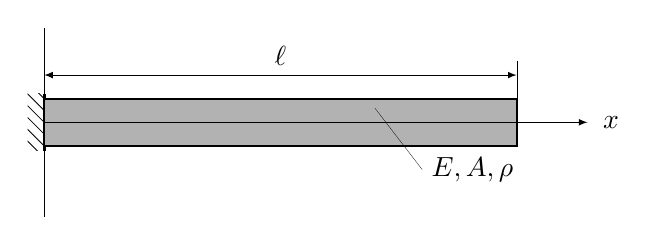
\begin{tikzpicture}[scale=0.6]
      \point{a}{0}{0};
      \support {3}{a}[270];
      % Draw the rectangle
      \filldraw[fill=gray!60, draw=black,thick] (0,-0.5) rectangle (10,0.5);
      %axis
      \draw[-latex, ultra thin] (0,0) -- (11.5,0);
      \draw[, ultra thin] (0,-2) -- (0,2);
      \node at (12,0) {\(x\)};
      % length
      \draw[ultra thin] (10,0) -- (10, 1.3) ;
      \draw[latex-latex, ultra thin]  (0,1)  to node[sloped,midway,above] {$\ell$}(10,1) ;
      \draw[ultra thin]  (7,0.3) -- (8,-1) node[right]{$E,A,\rho$};
    \end{tikzpicture}
  \end{center}
  \vspace{0.3cm}
  \begin{block}{}
    Find $u_{1}\in C^2([0,\ell]\times[0,T])$ such that
    \[
      \partial_{x}\big(EA \partial_{x}u_{1}\big) = \rho A \ddot{u}_1
    \]
    \begin{multicols}{2}
      boundary conditions:
      \[
        \begin{aligned}
          u_1(0, t)                    & = 0 \\
          EA \partial_{x} u_1(\ell, t) & = 0 \\
        \end{aligned}
      \]
      initial conditions:
      \[
        \begin{aligned}
          u_1(x, 0)       & = u_0(x) \\
          \dot{u}_1(x, 0) & = v_0(x)
        \end{aligned}
      \]
    \end{multicols}
    \vspace{0.01cm}
  \end{block}
\end{frame}


\begin{frame}{Disclaimer - exact or closed-form solution}
  The strong form for longitudinal vibrations of a bar admits an exact solution in the following decoupled form
  $$u_{1}(x,t)=\sum_{k=1}^{\infty} v_{k}(x)\phi_{k}(t)$$
  where
  $$v_{k}(x)=\sin\Big(\frac{\pi(2k-1)}{2\ell}x\Big)$$
  $$\phi_{k}(t)=a_{k}\sin(\omega_{k}t)+b_{k}\cos(\omega_{k}t)$$
  \vspace{-0.3cm}
  \begin{block}{}
    $$\omega_{k}=\frac{\pi(2k-1)}{2\ell}\sqrt{\frac{E}{\rho}}$$
  \end{block}
  \begin{itemize}
    \item  $a_{k}$ and $b_{k}$ depends respectively on the initial conditions $u_{0}$ and $v_{0}$.
    \item $k$ represents a mode of vibration ($k=1$ first or \emph{fundamental} mode).
  \end{itemize}
\end{frame}

\section{Weak formulation of equilibrium equations}

\begin{frame}
  \frametitle{Road to weak formulation}
  \begin{itemize}
    \item Strong formulations lead to strong solutions in the sense that they require strong continuity in the field variables.
    \item The weak form is often expressed as an integral equation that requires weaker continuity on the variables.
    \item The weak form can be obtained using the \emph{Virtual Work Principle}.
  \end{itemize}
  \vspace{-3pt}\noindent{\color{darkred}\rule{\linewidth}{0.1mm}\vspace{3pt}}

  The weak form is obtained through the following steps:
  \begin{enumerate}
    \item Multiply each differential equation by an appropriate arbitrary function.
    \item Integrate over the space domain of the problem.
    \item Reduce the order of the involved derivatives using the divergence theorem.
    \item Apply the boundary conditions reasonably.
  \end{enumerate}
\end{frame}

\begin{frame}
  \small
  \frametitle{Derivation of weak formulation}
  \begin{enumerate}
    \item Introduce an admissible \textbf{virtual displacement}:
          $$\boldsymbol\delta\mathbf u(\mathbf x)=\begin{bmatrix}\delta u_1(\mathbf x)\\ \delta u_2(\mathbf x)\\ \delta u_3(\mathbf x) \end{bmatrix}$$
    \item Multiply the differential equation in the strong form by $\boldsymbol\delta\mathbf u^{T}$ and integrate it over $\Omega$:
          $$\int_\Omega\boldsymbol\delta\mathbf u^{T}(\boldsymbol\nabla^T\mathbf C\boldsymbol\nabla \mathbf u+\mathbf f)\, d\Omega=\int_\Omega\rho\boldsymbol\delta\mathbf u^{T}\mathbf{\ddot{u}}\, d\Omega$$
    \item Apply the divergence theorem to the first term:
          $$-\int_\Omega (\boldsymbol\nabla\boldsymbol \delta\mathbf u)^{T} \mathbf C\boldsymbol\nabla \mathbf u\, d\Omega+{\color{darkred}\int_\Gamma \boldsymbol\delta\mathbf u^{T} \mathbf N^T\mathbf C\boldsymbol\nabla \mathbf  u\, d\Gamma}+\int_\Omega \boldsymbol\delta\mathbf u^{T}\mathbf f\, d\Omega=\int_\Omega\rho\boldsymbol\delta\mathbf u^{T} \mathbf{\ddot{u}}\, d\Omega$$
    \item Use the boundary conditions: $\mathbf N^T\mathbf  C\boldsymbol\nabla\mathbf  u=\mathbf{\hat f}$ on  $\Gamma_\sigma$ and \textcolor{darkred}{\emph{impose} $\boldsymbol\delta\mathbf u=\mathbf 0$ on $\Gamma_{u}$}:
          $$-\int_\Omega (\boldsymbol\nabla \boldsymbol\delta\mathbf u)^{T} \mathbf C\boldsymbol\nabla \mathbf u\, d\Omega+{\color{darkred}\int_{\Gamma_{\sigma}} \boldsymbol\delta\mathbf u^{T} \mathbf{\hat f}\, d\Gamma}+\int_\Omega \boldsymbol\delta\mathbf u^{T}\mathbf f\, d\Omega=\int_\Omega\rho\boldsymbol\delta\mathbf u^{T} \mathbf{\ddot{u}}\, d\Omega$$
  \end{enumerate}
\end{frame}

\begin{frame}
  \frametitle{Functional spaces}
  \begin{block}{}
    To ensure the integrals remain finite, we impose that:
    $$\mathbf u\in\mathcal U\qquad\mbox{and}\qquad \boldsymbol\delta\mathbf u\in\mathcal V$$
    \vspace{-1cm}
    \begin{align*}
      \mathcal U & =\big\{\mathbf u(\cdot,t)\in H^1(\Omega,\mathbb R^{3})\ |\ \mathbf u(\cdot,t)=\mathbf{\hat u}\ \mbox{on}\ \Gamma_u\ \forall t\in]0,T[\big\} \\
      \mathcal V & =\big\{\mathbf v\in H^1(\Omega,\mathbb R^{3})\ |\ \mathbf v=\mathbf 0\ \mbox{on}\ \Gamma_u\big\}
    \end{align*}
  \end{block}
  \vspace{-0.1cm}
  \begin{itemize}
    \item Recall that $H^1(\Omega)$ is the Sobolev space defined as
          $$H^1(\Omega)=\big\{\mathbf w\in L^2(\Omega,\mathbb R^{3})\ |\ \int_\Omega(\boldsymbol\nabla \mathbf w)^{T}\boldsymbol\nabla \mathbf w \ d\Omega<\infty \big\}.$$
    \item Note that the difference between spaces $\mathcal U$ and $\mathcal V$ is that only the functions in $\mathcal U$ are time-dependent.
    \item The spaces are designed to incorporate \emph{only} the displacement boundary condition on $\Gamma_{u}$.
  \end{itemize}
  \vspace{0.3cm}
\end{frame}

{\setbeamercolor{background canvas}{bg=darkred}
\setbeamercolor{block body}{bg=darkred,fg=white}
\setbeamercolor{itemize item}{fg=white}
\begin{frame}{Weak form of elastodynamics}
  \begin{block}{}
    Given $\Omega$, $\Gamma$, $\mathbf C$, $\rho$, $\mathbf f$, $\mathbf{\hat u}$, $\mathbf{\hat f}$, $\mathbf u_{0}$, $\mathbf v_{0}$ as in the previous slide, find the displacement $\mathbf u\in \mathcal U$ such that  that for any virtual displacement $\boldsymbol\delta\mathbf u\in \mathcal V$ we have
    $$\int_\Omega (\boldsymbol\nabla \boldsymbol\delta\mathbf u)^{T} \mathbf C\boldsymbol\nabla \mathbf u\, d\Omega+\int_\Omega\rho\, \boldsymbol\delta\mathbf u^{T}\mathbf{\ddot{u}}\, d\Omega=\int_{\Gamma_\sigma} \boldsymbol\delta\mathbf u^{T}\mathbf{\hat f} \, d\Gamma+\int_\Omega \boldsymbol\delta\mathbf u^{T}\mathbf f\, d\Omega,$$
    {\small$$\begin{rcases}\begin{aligned}
               & \mathbf u=\mathbf u_0\hspace{0.3cm}       & \text{for } t=0 \hspace{0.3cm} \\
               & \mathbf{\dot u}=\mathbf v_0\hspace{0.3cm} & \text{for } t=0\hspace{0.3cm}
            \end{aligned}
          \end{rcases}\text{Initial conditions}$$}
  \end{block}
\end{frame}
}

\section{Example 1: longitudinal vibrations of bars}

\begin{frame}{Strong form for longitudinal vibrations of bars (reminder)}
  \begin{columns}
    \column{0.65\textwidth}
    \begin{center}
      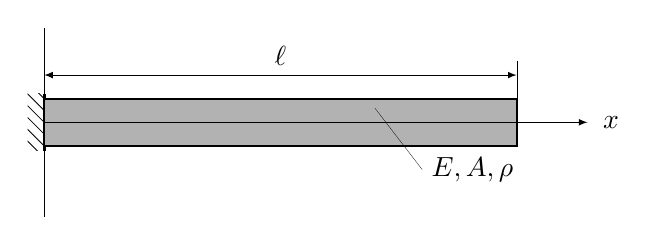
\begin{tikzpicture}[scale=0.6]
        \point{a}{0}{0};
        \support {3}{a}[270];
        % Draw the rectangle
        \filldraw[fill=gray!60, draw=black,thick] (0,-0.5) rectangle (10,0.5);
        %axis
        \draw[-latex, ultra thin] (0,0) -- (11.5,0);
        \draw[ultra thin] (0,-2) -- (0,2);
        \node at (12,0) {\(x\)};
        % length
        \draw[ultra thin] (10,0) -- (10, 1.3) ;
        \draw[latex-latex, ultra thin]  (0,1)  to node[sloped,midway,above] {$\ell$}(10,1) ;
        \draw[ultra thin]  (7,0.3) -- (8,-1) node[right]{$E,A,\rho$};
      \end{tikzpicture}
    \end{center}
    \column{0.5\textwidth}
    {\tiny \begin{itemize}
        \item $A$ cross-sectional area
        \item $E$ Young's modulus (isotropic bar)
        \item $\rho$ material density
        \item $\ell$ length
        \item $x$ axial coordinate
        \item $u_1(x,t)$ axial displacement
      \end{itemize}}
  \end{columns}
  \vspace{0.3cm}
  \begin{block}{}
    Find $u_{1}\in C^2([0,\ell]\times[0,T])$ such that
    \[
      \partial_{x}\big(EA \partial_{x}u_{1}\big) = \rho A \ddot{u}_1
    \]
    \begin{multicols}{2}
      boundary conditions:
      \[
        \begin{aligned}
          u_1(0, t)                    & = 0 \\
          EA \partial_{x} u_1(\ell, t) & = 0 \\
        \end{aligned}
      \]
      initial conditions:
      \[
        \begin{aligned}
          u_1(x, 0)       & = u_0(x) \\
          \dot{u}_1(x, 0) & = v_0(x)
        \end{aligned}
      \]
    \end{multicols}
    \vspace{0.01cm}
  \end{block}
\end{frame}

\begin{frame}
  \small
  \frametitle{Derivation of weak form for longitudinal vibrations of bars}
  \begin{enumerate}
    \item Define the virtual displacement $\delta u_{1}$ so that $\delta u_{1}\in H^{1}(]0,\ell[)$ and ${\color{darkred}\delta u_{1}(0)=0}$.
    \item Multiply the differential equation by the virtual displacement and integrate it over the intreval $]0,\ell[$.
          $$\int_0^\ell \partial_x\big(EA \partial_x u_1\big)\delta u_1\ dx=\int_0^\ell\rho A \ddot{u_1}\delta u_1\ dx.$$
    \item Use the integration by parts formula on the left hand side:
          $$-\int_0^\ell EA\, \partial_{x} u_1\,\partial_{x}(\delta u_1)\ dx+{\color{darkred}\big[EA \partial_{x} u_1\delta u_1\big]_0^\ell}=\int_0^\ell\rho A \ddot{u_1}\delta u_1\ dx.$$
    \item Make use of the boundary condition $EA\partial_{x}u_1(\ell,t) = 0$ and $\delta u_{1}(0)=0$ to simplify
          $$-\int_0^\ell EA\, \partial_{x} u_1\,\partial_{x}(\delta u_1)\ dx =\int_0^\ell\rho A \ddot{u_1}\delta u_1\ dx.$$
  \end{enumerate}
\end{frame}

\begin{frame}{Weak form for longitudinal vibrations of bars}
  \begin{block}{}
    Find $u_{1}\in \mathcal U$ such that for any $\delta u_1\in\mathcal V$ we have
    \[
      \int_0^\ell EA\, \partial_{x} u_1\,\partial_{x}(\delta u_1)\ dx +\int_0^\ell\rho A \ddot{u}_1\delta u_1\, dx=0,
    \]
    {\small$$\begin{rcases}\begin{aligned}
           & u_1=u_0\hspace{0.3cm}        & \text{for } t=0 \hspace{0.3cm} \\
           & {\dot u}_1=v_0\hspace{0.3cm} & \text{for } t=0\hspace{0.3cm}
        \end{aligned}
      \end{rcases}\text{Initial conditions}$$}
  \end{block}

  Recall:
  \begin{align*}
    \mathcal U & =\big\{u_{1}(\cdot,t)\in H^1(]0,\ell[)\ |\  u_1(0,t)=0\ \forall t\in]0,T[\big\} \\
    \mathcal V & =\big\{\delta u_{1}\in H^1(]0,\ell[)\ |\ \delta u_{1}(0)=0\big\}
  \end{align*}
\end{frame}


\section{Example 2: transversal vibrations of beams}

\begin{frame}
  \frametitle{Transversal vibrations of beams}
  \footnotesize\textbf{Kinematic assumptions:}
  \begin{itemize}
    \item The analysis will be restricted to the dynamic behavior of the beam in the $O(x,y)$ plane.
    \item  A normal cross-section to the neutral fiber remains planar after deformation, but not
          necessarily orthogonal to it
    \item  Shear strain $\varepsilon_{12}$ are taken into account (Timoshenko or thick beam).
  \end{itemize}
  \vspace{-0.3cm}
  \begin{columns}
    \column{0.6\textwidth}
    \begin{center}
      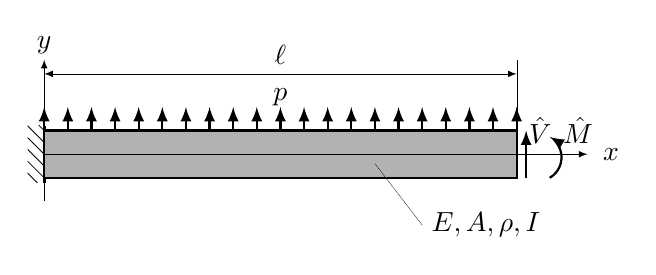
\begin{tikzpicture}[scale=0.6]
        \point{a}{0}{0.3};
        \support {3}{a}[270];
        % Draw the rectangle
        \filldraw[fill=gray!60, draw=black,thick] (0,0) rectangle (10,1);
        % Add the p vector
        \foreach \i in {0,...,20}
          {
            \draw[-latex, thick] (0.5*\i,1)-- (0.5*\i,1.5);
          }
        \node at (5,1.7) {\(p\)};
        %axis
        \draw[-latex, ultra thin] (0,0.5) -- (11.5,0.5);
        \draw[-latex, ultra thin] (0,-0.5) -- (0,2.5);
        \node at (12,0.5) {\(x\)};
        \node at (0,2.8) {\(y\)};
        % length
        \draw[ultra thin] (10,0) -- (10, 2.5) ;
        \draw[latex-latex, ultra thin]  (0,2.2)  to node[sloped,midway,above] {$\ell$}(10,2.2) ;
        % M and V 
        \draw[-latex, thick] (10.7,0) arc (-60:60:0.5);
        \node at (10.5,1) {\(\hat V\)};
        \draw[-latex, thick] (10.2,0) -- (10.2,1);
        \node at (11.3,1) {\(\hat M\)};
        \draw[ultra thin]  (7,0.3) -- (8,-1) node[right]{$E,A,\rho,I$};
      \end{tikzpicture}
    \end{center}
    \column{.25\textwidth}
    {\tiny \textbf{Model parameters:}
      \begin{itemize}\setlength\itemsep{0.05em}
        \item $A$ cross-sectional area
        \item $E$ Young's modulus
        \item $\rho$ material density
        \item $I$ moment of inertia
        \item $\ell$ length
      \end{itemize}}
    \column{.25\textwidth}
    {\tiny \textbf{Loads:}
      \begin{itemize}\setlength\itemsep{0.05em}
        \item  $\hat M$  bending moment \\ at free end
        \item  $\hat V$ shear force at \\ free end
        \item $p$ distributed transversal load
      \end{itemize}
    }
  \end{columns}
  \begin{block}{Variables}
    \begin{multicols}{2}
      \begin{itemize}\setlength\itemsep{0.05em}
        \item $u_{1}(x,y,t)$ axial displacement
        \item $u_{2}(x,y,t)$ transversal displacement\vspace{.1cm}
      \end{itemize}
    \end{multicols}
  \end{block}
\end{frame}

\begin{frame}
  \frametitle{Strain-displacement relationships}
  \vspace{-0.5cm}
  {\small
    \begin{itemize}
      \item   Introduce an auxiliary variable $\theta_{3}(x,t)$ representing the total rotation of the section around the $Oz$ axis:
            $$u_{1}(x,y,t)=-y\theta_{3}(x,t).$$
      \item Assume $u_{2}(x,y,t)=u_{2}(x,t)$ i.e. independent of $y$.
    \end{itemize}
  }
  \vspace{-0.3cm}
  \begin{columns}
    \column{0.4\textwidth}
    \begin{center}
      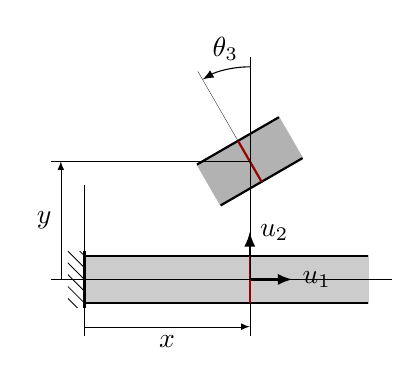
\begin{tikzpicture}[scale=0.6]
        \point{a}{0}{0.3};
        \support {3}{a}[270];
        % Draw the rectangle
        \filldraw[fill=gray!40, draw=gray!40,thick] (0,0) rectangle (6,1);
        \draw[thick](6,1)-- (0,1) -- (0,0)--(6,0);
        \draw[-latex,thick] (3.5,0.5) -- (4.4,.5) node[right]{$u_{1}$};
        \draw[-latex,thick] (3.5,0.5) -- (3.5,1.5) node[right]{$u_{2}$};
        \draw[darkred,thick] (3.5,0) -- (3.5,1);
        %deformed 
        \filldraw[fill=gray!60,draw=gray!60, rotate around={30:(3.5,3)}] (2.5,2.5) rectangle (4.5,3.5);
        \draw[thick,rotate around={30:(3.5,3)},shift={(0,-0.5)}](2.5,3)-- (4.5,3);
        \draw[thick,rotate around={30:(3.5,3)},shift={(0,0.5)}](2.5,3)-- (4.5,3);
        \draw[ultra thin,rotate around={30:(3.5,3)}](3.5,3)-- (3.5,5.2);
        \draw[darkred,thick,rotate around={30:(3.5,3)}](3.5,2.5)-- (3.5,3.5);
        \draw[-latex] (3.5,5) arc (90:120:2) node[midway,above] {$\theta_{3}$};
        %x1 and x2
        \draw[ultra thin] (3.5,-0.7) -- (3.5,0);
        \draw[-latex,ultra thin] (0,-0.5) to node[midway,below] {$x$} (3.5,-.5);
        \draw[ultra thin]  (-.7,3)-- (3.5,3);
        \draw[ultra thin] (3.5,5.2) -- (3.5,0.5);
        \draw[ultra thin] (-.7,0.5) -- (0,0.5);
        \draw[-latex,ultra thin] (-.5,.5) to node[midway,left] {$y$} (-.5,3);
        %axis
        \draw[ultra thin] (0,0.5) -- (6.5,0.5);
        \draw[ultra thin] (0,-0.7) -- (0,2.5);
      \end{tikzpicture}
    \end{center}
    \column{0.5\textwidth}
    \begin{block}{}
      \textbf{Normal strain :}
      $$\varepsilon_{11} =\partial_{x}u_{1}=-y\partial_{x}\theta_{3}$$
      \textbf{Shear strain :}
      $$ \varepsilon_{12} =\partial_{x}u_{2}+\partial_{y}u_{1}=\partial_{x}u_{2}-\theta_{3}$$
    \end{block}
  \end{columns}
\end{frame}

\begin{frame}
  \frametitle{Equilibrium equations}
  \begin{columns}
    \column{0.5\textwidth}
    \begin{center}
      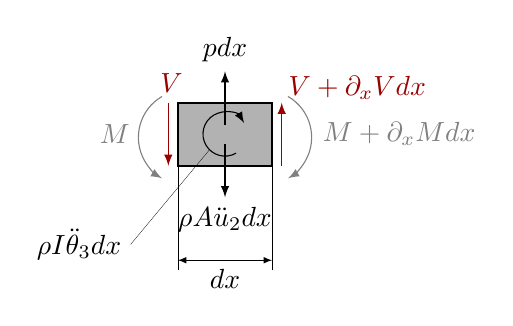
\begin{tikzpicture}[scale=0.4]
        % Draw the rectangle
        \filldraw[fill=gray!60, draw=black,thick] (0,0) rectangle (3,2);
        %axis
        \draw[ultra thin] (0,0) -- (0,-3.3);
        \draw[ultra thin] (3,0) -- (3,-3.3);
        \draw[ultra thin] (1,0.5) -- (-1.5,-2.5) node[left]{$\rho I\ddot \theta_{3}dx$};
        \draw[latex-latex,ultra thin] (0,-3) to node[midway,below] {$dx$} (3,-3);
        \draw[-latex]  (1.5,1.3)  -- (1.5,3) node[above] {$pdx$};
        \draw[-latex]  (1.5,.7)  -- (1.5,-1) node[below] {$\rho A\ddot u_{2}dx$};
        \draw[gray,-latex] (-0.5,2.2) arc (120:240:1.5);
        %M vectors 
        \node[gray] at (-2,1) {\(M\)};
        \draw[gray,-latex] (3.5,2.2) arc (60:-60:1.5);
        \draw (4.3,1) node[gray,right] {$M+\partial_{x}Mdx$};
        \draw[-latex] (1.85,.4) arc (300:30:0.7);
        % Add the V vectors
        \draw[darkred,latex-] (-0.3,0) -- (-0.3,2);
        \node[darkred,above] at (-0.2,2) {\(V\)};
        \draw[darkred,-latex] (3.3,0) -- (3.3,2);
        \node[darkred,above] at (5.7,1.8) {\(V+\partial_{x}Vdx\)};
      \end{tikzpicture}
    \end{center}
    \column{0.6\textwidth}
    \vspace{0.4cm}\newline \footnotesize Shear force $V$ and bending moment $M$ satisfy the following equations of motion:
    \begin{align*}
      \partial_{x}{\color{darkred}V}+p                & =\rho A\ddot u_{2}      \\
      -\partial_{x}{\color{gray}M}+{\color{darkred}V} & =\rho I\ddot \theta_{3} \\
    \end{align*}
  \end{columns}
  \vspace{.2cm}
  \footnotesize
  Since normal and shear stresses are $\sigma_{11}=E\varepsilon_{11}$ and $\sigma_{12}=G\varepsilon_{12}$ where $E$ is the Young's modulus and $G$ is the shear modulus, then
  \begin{align*}
    {\color{darkred}V} & =\int_{A}\sigma_{12}\, dA=kGA\varepsilon_{12}={\color{darkred} kGA(\partial_{x}u_{2}-\theta_{3})}   \\
    {\color{gray}M}    & =\int_{A} y\sigma_{11}\, dA=\int_{A}yE\varepsilon_{11}\, dA={\color{gray}-EI\partial_{x}\theta_{3}}
  \end{align*}
  where the constant $k$ is the shear correction factor (parabolic distribution of shear stresses).
\end{frame}

\begin{frame}
  \frametitle{Strong form for transversal vibrations of beams}
  \small The strong form for transversal vibrations of beams consists of finding the functions $u_{2}\in C^2([0,\ell]\times[0,T])$ and $\theta_{3}\in C^2([0,\ell]\times[0,T])$ such that the following equilibrium equations, boundary and initial conditions are satisfied.
  \begin{block}{Equilibrium equations}
    \vspace{-.5cm}
    \begin{align*}
      \partial_{x}\big({\color{darkred}kGA(\partial_{x}u_{2}-\theta_{3})}\big)+p                                      & =\rho A\ddot u_{2}      \\
      \partial_{x}\big({\color{gray}EI\partial_{x}\theta_{3}}\big)+{\color{darkred}kGA(\partial_{x}u_{2}-\theta_{3})} & =\rho I\ddot \theta_{3} \\
    \end{align*}
    \vspace{-1cm}\newline\small In matrix form:
    $$\underbrace{\begin{bmatrix}
          \partial_{x} & 0            \\
          1            & \partial_{x}
        \end{bmatrix}}_\text{$\nabla_{\sigma}^{T}$}
      \underbrace{\begin{bmatrix}
          kGA & 0  \\
          0   & EI
        \end{bmatrix}}_\text{$\mathbf C$}
      \underbrace{\begin{bmatrix}
          \partial_{x} & -1           \\
          0            & \partial_{x}
        \end{bmatrix}}_\text{$\nabla_{u}$}
      \underbrace{\begin{bmatrix}
          u_{2} \\
          \theta_{3}
        \end{bmatrix}}_\text{$\mathbf u$}
      +
      \underbrace{\begin{bmatrix}
          p \\
          0
        \end{bmatrix}}_\text{$\mathbf f$}
      =
      \underbrace{\begin{bmatrix}
          \rho A & 0      \\
          0      & \rho I
        \end{bmatrix}}_\text{$\mathbf M$}
      \underbrace{\begin{bmatrix}
          \ddot u_{2} \\
          \ddot \theta_{3}
        \end{bmatrix}}_\text{$\mathbf{\ddot u}$}
    $$
    $$\nabla_{\sigma}^{T}\mathbf C\nabla_{u}\mathbf u+\mathbf f=\mathbf {M \ddot u}$$
  \end{block}
\end{frame}

\begin{frame}
  \begin{block}{Boundary conditions}
    \begin{columns}
      \column{0.4\textwidth}
      \[
        \begin{aligned}
           & u_2(0, t) = 0 \quad        &  & \\
           & \theta_{3}(0, t) = 0 \quad &  & \\
        \end{aligned}
      \]
      \column{0.6\textwidth}
      \[
        \begin{aligned}
           & kGA \big(\partial_{x}u_{2}(\ell, t)-\theta_{3}(\ell, t) \big)= \hat V &  & \\
           & EI \partial_{x}\theta_{3}(\ell, t)=\hat M                             &  & \\
        \end{aligned}
      \]
    \end{columns}
    \vspace{.2cm}\small In matrix form: let $\hat{\mathbf{f}}=[\hat V,\, \hat M]^T$ then
    $$\begin{aligned}
        \mathbf u(0,t)                        & =\mathbf 0       \\
        \mathbf C\nabla_{u} \mathbf u(\ell,t) & =\mathbf{\hat f} \\
      \end{aligned}$$
  \end{block}

  \begin{block}{Initial conditions}
    \begin{columns}
      \column{0.5\textwidth}
      \[
        \begin{aligned}
           & u_2(x, 0) = u_{0}(x) \quad             &  & \\
           & \theta_{3}(x, 0) = \theta_{0}(x) \quad &  & \\
        \end{aligned}
      \]
      \column{0.5\textwidth}
      \[
        \begin{aligned}
           & \dot u_2(x, 0) = v_{0}(x) \quad           &  & \\
           & \dot \theta_{3}(x, 0) = \phi_{0}(x) \quad &  & \\
        \end{aligned}
      \]
    \end{columns}
    \vspace{.2cm}\small In matrix form:  $\mathbf{u_{0}}=[u_0,\, \theta_0]^T$ and $\mathbf{v_{0}}=[v_0,\, \phi_0]^T$ then
    $$\begin{aligned}
        \mathbf u(x,0)       & =\mathbf{u_{0}} \\
        \mathbf{\dot u}(x,0) & =\mathbf{v_{0}}
      \end{aligned}$$
  \end{block}
\end{frame}

\section{Complementary topics}

\begin{frame}{Constitutive material matrix for isotropic materials}
Recall that the constitutive material matrix is defined as $\mathbf C= \mathbf S^{-1}$ and for isotropic material 
  \vspace{0.2cm}
  {\small $$\mathbf S=\begin{bmatrix} 1/E & -\nu/E & -\nu/E & 0 & 0 & 0 \\  -\nu/E & 1/E  & -\nu/E  & 0 & 0 & 0 \\ -\nu/E & -\nu/E & 1/E & 0 & 0 & 0 \\ 0 & 0 & 0 & 1/G & 0 & 0 \\ 0 & 0 & 0 & 0 & 1/G & 0 \\ 0 & 0 & 0 & 0 & 0 & 1/G \end{bmatrix}$$ }
    {\small thus 
  $$  \mathbf C =
\frac{E}{(1+\nu)(1-2\nu)}
\begin{bmatrix}
1-\nu&\nu&\nu&0&0&0\\
\nu&1-\nu&\nu&0&0&0\\
\nu&\nu&1-\nu&0&0&0\\
0&0&0&\frac{1-2\nu}{2}&0&0\\
0&0&0&0&\frac{1-2\nu}{2}&0\\
0&0&0&0&0&\frac{1-2\nu}{2}
\end{bmatrix}$$}
\end{frame}

\begin{frame}{Normal and shear stresses}
  \begin{columns}[T,onlytextwidth]
    \begin{column}{0.5\textwidth}
      \begin{block}{Normal stresses $\sigma_{ii}$}
        A normal stress acts \alert{perpendicular} to the
        section plane.
        \begin{itemize}
          \item $\sigma_{ii}>0$: \textbf{tension}
          \item $\sigma_{ii}<0$: \textbf{compression}
        \end{itemize}
      \end{block}

      \begin{block}{Shear stresses $\tau_{ij}$}
        A shear stress acts \alert{tangentially} to the
        section plane.
        \begin{itemize}
          \item Produces \textbf{sliding} between adjacent material planes.
        \end{itemize}
      \end{block}
    \end{column}

    \begin{column}{0.4\textwidth}
      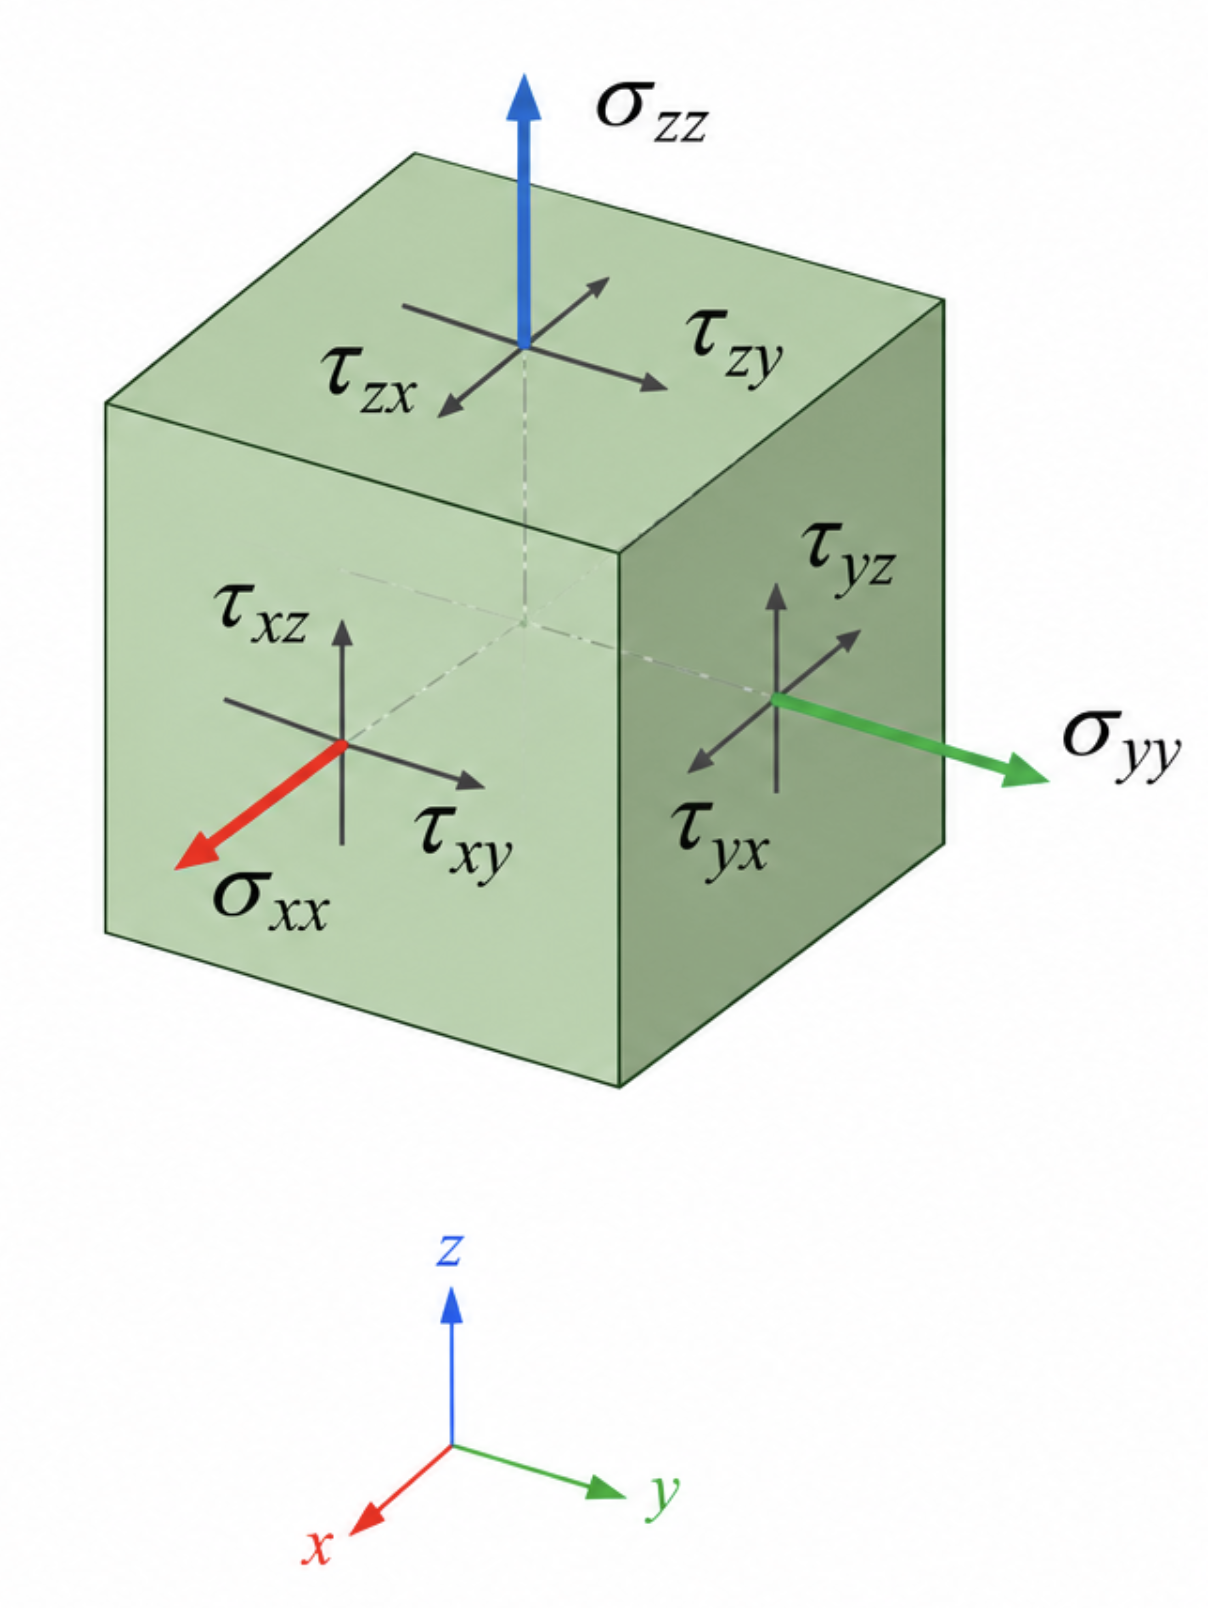
\includegraphics[width=0.9\textwidth]{../images/normalandshearstresses.png}
    \end{column}
  \end{columns}
\end{frame}

\begin{frame}{Principal stresses}
  \begin{block}{}\small Normal and shear stresses depend on the orientation of the section plane. Principal stresses are the normal stresses in the particular orientation for which all shear stresses vanish.
  \end{block}

  \begin{columns}[T]
    % ============================================================
    % LEFT COLUMN
    % ============================================================
    \begin{column}{0.48\textwidth}

      \large\textbf{Stress state at a material point}

      \vspace{0.15cm}

      \begin{itemize}

        \item \small In 3D, the stress state is completely described by
              \[
                \boxed{
                  \boldsymbol{\sigma}
                  =
                  \begin{pmatrix}
                    \sigma_{xx} & \tau_{xy}   & \tau_{xz}   \\
                    \tau_{xy}   & \sigma_{yy} & \tau_{yz}   \\
                    \tau_{xz}   & \tau_{yz}   & \sigma_{zz}
                  \end{pmatrix}
                }
              \]


        \item \small From moment equilibrium,
              \[
                \tau_{ij}=\tau_{ji}
              \]
              hence there are only \textbf{6 independent stresses}.

      \end{itemize}

    \end{column}

    % ============================================================
    % RIGHT COLUMN
    % ============================================================
    \begin{column}{0.50\textwidth}

      \large\textbf{Principal stresses}

      \vspace{0.05cm}

      \begin{itemize}
        \item \small There exists a coordinate system in which
              \[
                \tau_{xy}=\tau_{xz}=\tau_{yz}=0
              \]

        \item \small The remaining normal stresses are the
              principal stresses:
              \[
                \sigma_1,\quad\sigma_2,\quad\sigma_3
              \]

        \item \small They are the eigenvalues of the stress tensor:
              \[
                \boldsymbol{\sigma}\mathbf n_i
                =
                \sigma_i\mathbf n_i
              \]
      \end{itemize}
    \end{column}
  \end{columns}
\end{frame}

\begin{frame}{Strength hypotheses / equivalent stresses}

  \begin{itemize}

    % ------------------------------------------------------------
    % von Mises
    % ------------------------------------------------------------
    \item \textbf{von Mises stress for ductile materials}

          \vspace{-0.1cm}

          \[
            \sigma_{\mathrm{eq}}
            =
            \sqrt{
              \frac{
                (\sigma_1-\sigma_2)^2
                +
                (\sigma_2-\sigma_3)^2
                +
                (\sigma_3-\sigma_1)^2
              }{2}
            }
          \]

          Ductile material is still elastic or hasn't started to yield if $\sigma_{\mathrm{eq}} < \sigma_F$, where $\sigma_F$ is the yield strength of the material.

          % ------------------------------------------------------------
          % Tresca
          % ------------------------------------------------------------
    \item \textbf{Tresca stress for ductile materials}
          \[
            \sigma_{\mathrm{Tresca}}
            =
            \max
            \left(
            |\sigma_1-\sigma_2|,
            |\sigma_2-\sigma_3|,
            |\sigma_3-\sigma_1|
            \right)
          \]

          % ------------------------------------------------------------
          % Mohr-Coulomb
          % ------------------------------------------------------------
    \item \textbf{Mohr--Coulomb for brittle materials}
          \[
            \frac{\sigma_1}{\sigma_{\max,\mathrm{tens}}}
            +
            \frac{\sigma_3}{\sigma_{\max,\mathrm{comp}}}
            <1
          \]

          % ------------------------------------------------------------
          % Maximum principal stress
          % ------------------------------------------------------------
    \item \textbf{Maximum principal stress criterion for brittle materials}
          \[
            \sigma_1 < \sigma_{\max,\mathrm{tens}}
          \]
  \end{itemize}
\end{frame}

\end{document}





